\documentclass{xduugmr}

\usepackage{float} % \begin{figure}[H] 图片紧随文字
\usepackage{booktabs}
\usepackage{graphicx}
\usepackage{longtable}

\usepackage{expl3}

\ExplSyntaxOn
\cs_set:Npn \figurename { 图 }
\cs_set:Npn \tablename { 表 }
\ExplSyntaxOff

\xdusetup{
style = { 
    cjk-font = fandol, 
    latin-font = gyre,
    bib-backend = biblatex % -> biber
},
info = {
    department = {计算机科学与技术院},
    major = {计算机科学与技术},
    author = {江志航},
    supervisor = {霍秋艳},
    class = {2103018},
    student-id = {20009100359},
    bib-resource = {reference.bib},
}
}

\begin{document}

\section{毕业设计工作是否更换题目及是否按开题报告预定的内容及进度安排进行}

不更换题目,按开题报告预定的内容及进度安排进行。

\section{目前已完成的研究工作及结果(内容要详实充分)}

\subsection{研究背景与意义}

在全球人口持续增长以及人们对农产品品质与安全关注度日益提升的大背景下,农业的发展面临着前所未有的挑战与机遇。智慧农业作为一种融合了现代信息技术、生物技术、工程技术等多学科技术的新型农业发展模式\cite{赵春江2021智慧农业的发展现状与未来展望},正逐渐成为推动农业现代化进程的关键力量。它通过对农业生产过程中的各种数据进行实时采集、传输、分析和处理,实现了农业生产的精准化、智能化和自动化管理\cite{李道亮2012物联网与智慧农业},有效提高了农业生产效率、降低了生产成本、保障了农产品质量安全,为解决当前农业发展面临的诸多问题提供了新的思路和方法。

果实称重作为精准农业的重要环节,对于农业生产管理和决策具有不可或缺的作用\cite{罗锡文2016信息技术提升农业机械化水平}。准确的果实称重数据能够为农民提供有关农作物产量的精确信息,帮助他们及时了解农作物的生长状况\cite{翁杨2019基于深度学习的农业植物表型研究综述},进而合理安排农事活动,如施肥、灌溉、病虫害防治等,以提高农作物的产量和质量。通过对果实称重数据的分析,还可以为农产品的市场定价、销售策略制定以及供应链管理提供有力的数据支持,有助于优化农产品的流通环节,提高农业经济效益\cite{Lipcsei2021AnalysisOA}。在水果采摘环节,精确的称重能够实现水果按重量分级,满足不同消费者的需求,提升水果的市场竞争力\cite{Ji2019};在农产品加工行业,准确的原料称重是保证产品质量一致性和生产工艺稳定性的关键因素。

然而,传统的果实称重方式主要依赖人工操作,存在着诸多明显的不足。人工称重效率低下,在大规模的农业生产中,需要耗费大量的人力和时间,尤其是在果实收获季节,繁重的称重工作往往使人力成本大幅增加\cite{Jiang2012}。人工称重容易受到人为因素的影响,导致称重数据的准确性和可靠性难以保证,如操作人员的疲劳、疏忽以及读数误差等,都可能使称重数据出现偏差,从而影响后续的生产决策\cite{Chen2002}。同时,这种传统的称重方式在数据记录和管理上也较为繁琐,难以实现数据的实时共享和高效分析,无法满足现代精准农业对数据快速处理和深度挖掘的需求\cite{Widagdo2020RecordingSO}。

随着云计算、物联网、大数据等信息技术的飞速发展,将这些先进技术应用于农业领域,构建农业果实称重云端系统,成为推动农业数字化转型的必然趋势。云端系统能够实现果实称重数据的实时采集、传输和存储,打破了时间和空间的限制,使得农民和农业管理者可以随时随地获取和管理称重数据\cite{李道亮2012物联网与智慧农业}。通过对海量称重数据的分析挖掘,云端系统能够为农业生产提供更加科学、精准的决策支持,如产量预测、市场趋势分析等,有助于农业生产者更好地应对市场变化,降低生产风险\cite{韩佳伟2022装备与信息协同促进现代智慧农业发展研究}。云端系统还可以与其他农业信息化系统进行集成\cite{刘洋2013基于物联网与云计算服务的农业温室智能化平台研究与应用术},实现农业生产全过程的信息化管理,进一步提升农业生产的智能化水平,推动智慧农业的发展。

基于以上背景,本文研究将深入调研农村电子秤称重的流程,了解农场电子秤称重数据的特点和应用场景,设计并利用软件技术,实现对农场电子秤称重数据的实时采集,并通过云端数据库存储和分析,实现对数据的实时共享和高效分析,为农业生产提供更加科学、精准的决策支持。同时系统还将提供与称重数据相关的果实、员工、采摘作业等信息的管理和可视化展示,帮助农业生产者更好地管理农业生产环境,提高农业生产效率。

\subsection{国内外研究现状}

在国外,智慧农业的发展起步较早,农业果实称重技术与云端系统的应用研究也取得了较为显著的成果。美国作为农业科技强国,在农业领域广泛应用了先进的传感器技术和物联网技术\cite{赵春江2021智慧农业的发展现状与未来展望}。例如,一些大型农场采用了高精度的电子称重传感器,能够实时采集果实的重量数据,并通过无线传输技术将数据发送至云端服务器\cite{陈学庚2020农业机械与信息技术融合发展现状与方向}。在加利福尼亚州的部分果园,利用智能称重设备与云端系统相结合,实现了对水果采摘过程的精准监控和管理\cite{Ampatzidis2011},农场主可以通过手机或电脑随时查看每个采摘区域的果实产量、重量分布等信息,从而及时调整采摘计划和资源分配。美国还在研发基于图像识别和深度学习的果实称重与分级系统,通过对果实图像的分析\cite{Anisha2019FruitRU},不仅能够准确获取果实的重量,还能对果实的品质进行评估,进一步提高了果实称重与分级的智能化水平。

欧洲在农业果实称重云端系统的研究和应用方面也处于领先地位。德国的一些农业企业开发了集成化的农业生产管理平台,其中包含了果实称重与数据分析模块\cite{Yin2020}。这些平台通过与各种农业设备的连接,实现了果实称重数据的自动采集和实时上传,同时利用大数据分析技术对数据进行深度挖掘,为农业生产提供了全面的决策支持,如预测产量、优化种植方案等\cite{Phate2021}。荷兰则专注于温室农业中的果实称重技术研究,通过在温室中安装传感器网络,实现了对温室作物果实生长过程的全程监测和重量测量\cite{Graaf2004},利用云端系统对数据进行分析和管理,为温室作物的精准种植和高效管理提供了有力保障。

在国内,随着智慧农业的快速发展,农业果实称重云端系统的研究和应用也逐渐受到重视。近年来,国内高校和科研机构在该领域开展了大量的研究工作,并取得了一系列的成果。一些研究团队开发了基于物联网的果实称重系统,通过将电子秤与物联网模块相结合,实现了果实称重数据的无线传输和远程监控\cite{Zhu2013}。在山东的一些果园,应用了这种物联网称重系统,果农可以通过手机 APP 实时查看果实的称重数据,方便了果实采摘和销售管理\cite{Gao2023}。国内企业也积极投入到农业果实称重云端系统的研发和推广中。一些科技公司推出了针对不同农业场景的果实称重解决方案\cite{Ningbo2019},不仅提供了硬件设备,还开发了相应的软件平台,实现了数据的云端存储、分析和可视化展示,帮助农业生产者更好地管理果实称重数据,提高农业生产效率。

然而,目前国内外的研究仍存在一些不足之处。一方面,部分果实称重系统的精度和稳定性有待提高,在复杂的农业生产环境中,容易受到温度、湿度、电磁干扰等因素的影响,导致称重数据出现偏差\cite{汤建华2018}。另一方面,现有的云端系统在数据安全和隐私保护方面还存在一定的风险,随着农业数据的价值不断提升,如何保障数据的安全传输和存储,防止数据泄露和篡改,成为亟待解决的问题。此外,不同地区和不同作物的果实称重需求存在差异,现有的系统在通用性和适应性方面还需要进一步优化,以满足多样化的农业生产需求,比如云端系统需要支持更多物联网通信协议,如 MQTT、HTTP、CoAP 等,以满足更多不同类型电子秤的通信需求。

\subsection{研究目标与内容}

本研究旨在设计并实现一个高效、稳定、功能强大的农业果实称重云端系统,以满足现代农业生产对果实称重数据精准管理和深度分析的需求。具体研究目标如下:

一、系统设计与实现:运用先进的信息技术,构建一个基于云端架构的农业果实称重系统,实现果实称重数据的实时采集、传输、存储和处理。确保系统具备良好的用户界面,操作简便,易于推广使用,为农业生产者和管理者提供便捷的服务。

二、多协议兼容与设备管理:使系统支持多种常见的电子秤通信协议,如 HTTP/HTTPS、MQTT、CoAP、STOMP 等,能够与市场上不同类型的电子秤设备进行无缝对接,实现数据的准确接收和解析。同时,提供完善的电子秤设备管理功能,包括设备注册、配置、状态监测等,方便用户对电子秤进行统一管理。

三、数据统计与导出:开发强大的数据统计和导出功能,支持从批次、采摘人员、时间等多个维度对称重数据进行统计,生成报表和折线图,便于管理者更直观地分析数据,了解农村情况,从而更好地优化生产策略,提高经济效益。

四、系统性能优化与测试:对系统的性能进行全面优化,确保系统在高并发、大数据量的情况下能够稳定运行,具备良好的响应速度和扩展性。通过一系列的性能测试,评估系统的可用性、每秒查询率(QPS)、并发用户数和响应时间等指标,验证系统是否满足设计要求。

围绕上述研究目标,本研究的主要内容包括以下几个方面:

一、系统架构设计:深入研究云计算、物联网、大数据等相关技术,结合农业果实称重的业务需求,设计出合理的系统架构。包括云端软件前端界面设计、电子秤终端模拟界面设计、后端服务架构、数据存储方案以及通信协议的选择等,确保系统的稳定性、可扩展性和安全性。

二、功能模块开发:根据系统设计方案,开发各个功能模块,主要包括工作服务模块、称重服务模块、用户管理模块、果实管理模块等。在开发过程中,遵循软件工程的原则,采用先进的开发框架和技术,确保代码的质量和可维护性。

三、性能测试与优化:制定详细的性能测试计划,运用专业的测试工具对系统进行性能测试,分析测试结果,找出系统存在的性能瓶颈。针对性能瓶颈,采取相应的优化措施,如优化数据库查询语句、调整服务器配置、采用缓存技术等,不断提升系统的性能。

\subsection{研究方法与技术路线}

本研究综合运用多种研究方法,以确保研究的科学性、全面性和实用性,包括具体文献研究法、案例分析法、系统开发方法、测试验证法。各研究方法具体内容如下:

一、文献研究法:广泛收集和查阅国内外关于智慧农业、果实称重技术、云计算、物联网等领域的相关文献资料,包括学术期刊论文、学位论文、研究报告、专利文献以及行业标准等。对这些文献进行系统梳理和分析,了解该领域的研究现状、发展趋势以及存在的问题,为本研究提供理论基础和研究思路,避免重复研究,确保研究的创新性和前沿性。通过对相关文献的研究,深入了解现有的果实称重技术和云端系统架构,为系统的设计与实现提供参考。

二、案例分析法:选取国内外具有代表性的农业果实称重项目和智慧农业应用案例进行深入分析,研究其系统架构、功能实现、应用效果以及面临的挑战等。通过案例分析,总结成功经验和不足之处,为本研究的农业果实称重云端系统的设计与优化提供实践参考。例如,对美国某大型农场采用的智能称重设备与云端系统相结合的案例\cite{Anisha2019FruitRU}进行分析,了解其在提高果实称重效率和管理水平方面的具体做法和成效,从中汲取有益的经验。

三、系统开发方法:依据软件工程的原理和方法,本项目将采用瀑布模型的开发方法来组织开发工作。瀑布模型又称生存周期模型,由 B.M.Boehm 提出,是软件工程的基础模型。其核心思想是按工序开发软件,将功能的分析、设计与实现分开,便于分工协作\cite{叶俊民2006软件工程}。农业果实称重云端系统的开发将采用结构化的分析与设计方法,把逻辑实现与物理实现分开,各项软件工程活动包括:制定开发计划、进行需求分析和说明、软件设计、程序编码、测试及运行维护。

四、测试验证法:运用专业的测试工具和方法,对开发完成的农业果实称重云端系统进行全面的测试。功能测试主要验证系统是否满足各项功能需求,如电子秤数据采集、数据传输、数据分析、报表生成等功能是否正常;性能测试主要评估系统在高并发、大数据量情况下的性能表现,包括系统的响应时间、吞吐量、并发用户数等指标;安全测试主要检测系统的安全性,如数据加密、用户认证、权限管理等方面是否存在漏洞。通过测试,及时发现系统存在的问题和缺陷,并进行优化和改进,确保系统能够稳定、可靠地运行。

本研究的技术路线主要包括需求分析、系统设计、功能模块开发、系统集成与测试、系统部署与应用以及研究总结与展望。下面对这些步骤进行具体阐述。

首先是需求分析,调研农业的实际生产流程,了解在果实称重管理方面的实际需求和业务流程,分析现有果实称重方式存在的问题和痛点,明确系统的功能需求、性能需求、安全需求以及用户体验需求等,整理相关的需求文档,为后续的系统设计提供依据。

接下来是系统设计。基于需求分析的结果,结合云计算、物联网、大数据等技术,进行农业果实称重云端系统的架构设计,确定系统的前端界面设计、后端服务设计、数据库设计、数据库存储方案以及通信协议等。根据需求文档所描述的业务流程,设计并书写接口文档,方便前后端的并行开发。对于具体的业务细节,可以利用 UML 图来描述业务的具体流程,比如可以使用时序图和活动图来描述称重的流程,以及使用类图来描述各个模块的关系。在前端设计中,注重用户界面的友好性和易用性,采用响应式设计,确保系统能够在不同设备上正常运行;在后端设计中,注重服务的高可用,提供响应速度良好的接口,提高系统的可扩展性和维护性;在数据库设计中,可以遵循改进后的新奥尔良方法(New Orleans Method),将数据库设计分为需求分析、概念结构设计、逻辑结构设计、物理结构设计、数据库实施和数据库运行和维护这六个阶段,设计出良好、可维护的数据库\cite{苗雪兰2001数据库系统原理及应用教程};在数据存储方面,选择合适的数据库管理系统,如关系型数据库和非关系型数据库相结合,以满足不同类型数据的存储需求;在通信协议方面,选用 HTTP、MQTT、CoAP、STOMP 等常见协议,确保电子秤与云端系统之间的数据传输稳定可靠。

完成系统设计之后,即可开始进行功能模块开发。根据系统设计方案,开发各个功能模块。利用前端开发技术,如 Vue、Vite、TypeScript 等,实现系统的前端界面,包括电子秤配置界面、数据查看界面、报表生成界面等;利用后端开发技术,如 Java、Spring Boot、Spring Security 等,实现系统的后端服务,包括工作服务模块、称重服务模块、用户管理模块、果实模块等;利用数据库开发技术,如 MySQL、Redis 等,实现数据的存储和管理;利用通信技术,如 MQTT 客户端库、HTTP 客户端库等,实现电子秤与云端系统之间的数据传输。

完成各个模块的开发之后,即可开始进行系统集成与测试。将开发完成的各个功能模块进行集成,搭建完整的农业果实称重云端系统。制定详细的测试计划,对系统进行全面的测试,包括单元测试、集成测试、系统测试和验收测试等。在测试过程中,记录测试结果,分析测试数据,及时发现并解决系统中存在的问题和缺陷。对系统的性能进行优化,如优化数据库查询语句、调整服务器配置、采用缓存技术等,提高系统的响应速度和吞吐量,确保系统能够满足实际应用的需求。

测试完成,确保没有问题之后,即可进行系统部署与应用。将测试通过的系统部署到生产环境中,进行实际应用。在应用过程中,收集用户的反馈意见,对系统进行持续优化和改进。对系统的应用效果进行评估,分析系统在提高果实称重效率、数据管理水平以及为农业生产决策提供支持等方面的作用,总结经验教训,为进一步完善系统和推广应用提供参考。

最后,进行研究总结与展望:对整个研究过程和结果进行总结,归纳研究成果和创新点,分析研究过程中存在的问题和不足之处,提出未来的研究方向和展望。为农业果实称重云端系统的进一步发展和应用提供理论支持和实践指导,推动智慧农业的发展。

通过以上研究方法和技术路线,本研究旨在构建一个高效、稳定、功能强大的农业果实称重云端系统,为现代农业生产提供有力的支持和保障。

\subsection{系统分析}

\subsubsection{系统功能需求分析}

本研究从实际农业生产流程出发,了解在果实称重管理方面的实际需求和业务流程,分析现有果实称重方式存在的问题和痛点,明确系统的功能需求、性能需求、安全需求以及用户体验需求等。

随着电子秤的推广,在智慧农场果蔬采摘称重是精准收获中重要的一环。而目前很大程度上仍然需要通过人工进行采摘,因此,需要对采摘果实进行称重记录、统计果蔬产量进行管理。传统的果实称重方式主要依赖人工操作,存在着诸多明显的不足。比如无法保证称重数据的准确性和可靠性,人工称重效率低下,数据记录和管理上也较为繁琐,难以实现数据的实时共享和高效分析,比如在一个大型农场信息管理系统中,通常需要对果实称重数据进行统计分析,生成报表,以便于管理者更好地了解农场的生产情况,从而更好地优化生产策略,提高经济效益。

针对以上需求背景,本研究从分析称重流程出发,逐步介绍系统所需要实现的功能点。下面开始模拟并分析称重的流程。

称重人员只需要将果实放上称重台,在终端通过刷卡认证并选择果实种类,然后等待称重数据上传。电子秤终端会自动读取电子秤的称重结果,然后生成更具体的数据信息,最后通过某种通信协议请求云端软件的服务地址,完成称重数据的存储。后台数据处理完成后,给前台反馈处理的结果。具体的称重流程时序图如图\ref{fig:称重流程时序图}所示。

\begin{figure}[H]
    \centering
    \includegraphics[width=0.8\linewidth]{../design/out/称重流程时序图.png}
    \caption{称重流程时序图}
    \label{fig:称重流程时序图}
\end{figure}

对于整个称重流程,有几个关键的判断节点需要注意。首先是员工认证,如果后台认证失败,员工不可进入果实选择界面;接着是称重数据的提交,在后台完成相关动作之后,需要返回给前台相应的提示信息;最后是提示员工是否继续称重,如果不继续称重,需要登出帐号,以确保数据安全,否则退回到果实选择界面。具体的称重流程活动图如图\ref{fig:称重流程活动图}所示。

\begin{figure}[H]
    \centering
    \includegraphics[width=0.8\linewidth]{../design/out/称重流程活动图.png}
    \caption{称重流程活动图}
    \label{fig:称重流程活动图}
\end{figure}

基于此称重流程,可以发掘出几个功能点,首先是用户管理,需要有一个用户管理模块,来完成称重人员的信息认证,除此之外,需要实现管理员和用户的角色区分,管理员可以执行对其他用户的管理功能,以及对诸如电子秤、采摘作业等的管理;其次是果实管理,发送的称重数据需要包括果实的种类,同时后续也需要根据果实的称重结果进行产量相关的统计;接着是工作管理,每次提交的称重数据,应该包含唯一确定一次采摘作业的编号,这样才可以达到分批次统计产量的目的;最后是称重相关的功能,包括电子秤管理和称重数据的处理,注意需要实现多种协议电子秤的兼容,包括 HTTP、CoAP、MQTT 等。

针对上述对称重流程的分析,本系统将会实现一个更加全面的农场信息管理系统,包括果实称重数据的实时采集、传输、存储和处理,果实、员工、采摘作业等信息的管理和可视化展示,帮助农业生产者更好地管理农业生产环境,提高农业生产效率。具体包括了用户管理模块、果实模块、工作服务模块、称重服务模块等。具体模块功能如工作分解结构图\ref{fig:工作分解结构图}所示。

\begin{figure}[H]
    \centering
    \includegraphics[width=0.8\linewidth]{../design/out/工作分解结构图.png}
    \caption{工作分解结构图}
    \label{fig:工作分解结构图}
\end{figure}

工作分解结构图\ref{fig:工作分解结构图}归纳了各个模块应该实现的功能。下面进行具体阐述:

一、用户管理模块,包含用户功能和管理员功能,用户在这个模块中,可以进行登录认证,以及对个人信息的修改。管理员是一种特殊的用户,除了普通用户所拥有的功能以外,管理员可以对其他用户进行增删改查操作。

二、果实模块,包含果实管理功能和果实统计功能。对于果实管理,管理员可以对果实信息进行维护,所有用户可以对果实进行查询。对于果实统计,管理员可以获取任一果实的年产量统计结果和分批作业的产量统计结果,这些统计结果需要支持导出为 Excel 并可以在前台通过折线图完成可视化功能。

三、工作服务模块,包含工作管理功能和工作分配功能。对于工作管理,管理员可以进行对采摘工作的查询和维护,这个采摘工作可以定义为某个时间段对某个果实的采摘作业。对于工作分配,管理员可以分配具体的采摘作业给某些员工,而员工可以查询到自己所负责的作业。

四、称重服务模块,包含电子秤管理功能、称重记录功能和统计分析功能。对于电子秤管理,管理员可以进行电子秤信息的维护和查询。对于称重记录,电子秤终端可以发送称重数据到云端软件,完成称重记录的存储。管理员可以针对任一电子秤,查询其历史称重数据。对于统计分析,员工可以查询自己各作业的采摘量。

分解完系统所涉及的功能模块后,再具体对系统中存在的角色以及它们与系统功能的关联进行阐述。下面通过用例图来对其进行解释,如图\ref{fig:核心功能用例图}所示。

\begin{figure}[H]
    \centering
    \includegraphics[width=0.8\linewidth]{../design/out/核心功能用例图.png}
    \caption{核心功能用例图}
    \label{fig:核心功能用例图}
\end{figure}

从用例图\ref{fig:核心功能用例图}可以知道,本系统存在三个角色:采摘员工、电子秤终端和农场管理员。采摘员工涉及三个方面的功能,包括用户服务、称重服务和数据可视化。电子秤终端则是一个特殊的角色,用来完成称重服务;农场管理员也涉及三个方面的功能,包括用户服务、数据可视化和农场管理。

\subsubsection{非系统功能需求分析}

非系统功能需求是指系统在使用过程中,除了实现基本功能外,还需要满足的一些性能、安全、可靠性、易用性等方面的需求。本系统的非系统功能需求主要包括以下几个方面:

\begin{enumerate}
    \item 高可用性:称重数据的提交和查询需要保证系统的高可用性,确保系统能够稳定运行,不会因为系统故障或网络中断导致数据丢失。
    \item 高性能:系统需要具备良好的性能,能够在高并发、大数据量的情况下保持稳定运行,具备良好的响应速度和吞吐量。
    \item 数据安全:系统需要保证称重数据的安全性,确保数据传输过程中的加密和解密,防止数据泄露和篡改。
    \item 易用性:系统需要具备良好的用户界面,操作简便,易于推广使用,用户可以快速上手,提高工作效率。
    \item 可扩展性:系统需要具备良好的可扩展性,能够支持多种电子秤通信协议,满足不同类型电子秤的通信需求。
\end{enumerate}

其中,尤其需要注意数据安全、高性能和高可用性。下面对这三个需求进行具体分析。

对于数据安全,首先需要确保所有称重数据的提交都是加密的,比如使用 HTTPS 代替 HTTP,来完成数据的通信;其次,对于数据库的访问,需要配置好用户名和密钥,禁止匿名访问;第三,存储在数据库的密钥需要加密,不可以明文存储;最后,对于一些数据处理中间件,如果涉及某些主题的订阅和消息发布,不同的消费者和生产者需要做好权限的控制,避免消息的错误发布和消费。

对于高性能,在农场称重的活动中,同一时间,可能有上万台设备在提交称重数据,这时候的 QPS 将是上万级别的,如果不能处理好称重数据的快速提交,将会对农业生产造成很大的影响。因此,需要确保系统的高可用性,可以采用一些消息队列来处理这个问题。

对于高可用性,如果在农场称重过程中,后台服务出现宕机的情况,那么将无法处理任何请求,这将对农业生产造成很大的影响。因此,需要确立好一个良好可伸缩的软件架构,在某台机器宕机的情况下,可以快速使用另一个机器进行服务,确保称重服务的高可用。

\subsection{系统可行性分析}

可行性分析是一门研究技术领域中经济问题和经济规律的科学,旨在探索在特定技术条件下如何提高经济效益。它是技术与经济的交叉领域,主要研究技术实施的经济效果以及技术与经济的最佳组合方案。首先,需要对系统进行全面的可行性分析,以确定系统是否能够实现,是否满足各方面的需求。可行性分析包括技术可行性、经济可行性、法律和社会可行性,还需考虑增加操作可行性的实际需求。

\subsubsection{操作可行性分析}

农业果实称重云端软件的操作界面设计力求简洁直观,简化操作流程,使其尽可能符合用户的使用习惯和业务需求。因此,操作人员只需经过简单的培训即可熟练使用,从而确保本系统在操作可行性方面不会存在任何问题。

\subsubsection{技术可行性分析}

农业果实称重云端软件属于信息管理系统,主要涉及数据库开发技术和前端操作界面的开发。当前,数据库开发技术已取得显著进步,结合本系统的应用范围和功能需求,采用合适的开发平台可以充分满足功能要求。此外,数据库开发与前端界面结合在信息管理系统领域已有众多成功案例,因此本系统在技术实现上是完全可行的。

系统的可行性分析主要从以下几个方面进行考虑:
	
\begin{enumerate}
    \item 安全性:
    为了确保系统的安全性,利用数据库技术,通过编写存储过程等手段,保障系统的并发性和恢复能力,同时有效防止通过SQL注入等技术对数据进行窃取和篡改。
    \item 可运行性:
    本系统作为一个小型管理系统,所需的资源消耗非常小,能够在较低配置的环境下稳定运行。
\end{enumerate}

\subsubsection{经济可行性分析}

由于本软件是一个小型的农业果实称重云端软件,因此其开发经费和投资较少,仅需一台普通的计算机即可完成开发。系统的开发过程并不复杂,操作尽可能保持简洁易用,具有良好的用户体验和实用性,因而在经济上具有合理性。

在系统开发方面,由一人独立完成,预计开发周期约为三个月。开发成本主要包括人工费用,此外还包括计算机和软件的投入成本。由于计算机和软件均可重复使用,采用自主开发方式不仅节省了费用,还能根据自身需求定制功能,并掌握完整的源代码,方便系统后续的扩展和维护。因此,从成本和效益的角度来看,开发农业果实称重云端软件是完全可行的。

\subsection{系统设计}

\subsubsection{系统设计模式}

在农业果实称重云端软件中,基于前后端分离的开发思想,采用了 Spring + Vue 的技术栈,基于 MVC(Model-View-Controller) 和 MVVM(Model-View-ViewModel) 的设计模式来完成开发。下面对这两种设计模式进行具体阐述。

在现代 Web 开发中,前后端分离已成为一种主流的架构模式。传统的 Web 开发通常采用服务端渲染(SSR)的方式,前端和后端集成在一起,由后端生成 HTML 页面并返回给浏览器,浏览器仅负责解析和展示页面内容。然而,随着 Web 技术的发展和前端框架(如 React、Vue.js、Angular)的广泛应用,前后端分离的架构逐渐成为主流。

在前后端分离架构下,前端和后端的开发、部署和运行环境是独立的,二者通过 API 进行通信。前端专注于页面的展示和交互,通过调用后端的接口获取数据和提交操作;后端则专注于业务逻辑的处理、数据存储和安全管理。通过这种分离,前后端可以独立开发、测试和部署,提高了开发效率和系统的扩展性。

在前后端分离的架构模式下,MVC 设计模式依然存在,但它的角色和应用场景发生了一些变化。前后端分离的架构通常意味着前端和后端的职责和运行环境是分开的,前端通过 API(通常是 RESTful 或 GraphQL)与后端进行通信。

后端依然可以使用 MVC 模式来处理请求和响应。具体来说,后端的 MVC 主要处理以下内容:
\begin{enumerate}
    \item Model:表示业务逻辑层或数据模型,通常是数据库实体或服务层中的数据对象。它负责处理数据存取、验证和计算等操作。
    \item View:在传统的 MVC 中,View 是用户界面部分,负责显示数据。而在前后端分离架构中,后端的 View 主要是指服务器端生成的 JSON 或 XML 数据,它不是直接渲染页面,而是以 API 的形式将数据返回给前端。
    \item Controller:处理客户端请求、调用相应的业务逻辑(Model),并最终返回一个响应。Controller 将从 Model 中获取数据,通常会将其转化为 JSON 格式并返回给前端。
\end{enumerate}

在这种情况下,后端的 MVC 模式 用于接收和处理 API 请求,完成业务逻辑并返回数据,而不直接负责页面渲染。后端的 Controller 负责接收前端发送的 HTTP 请求,调用 Model 层进行数据处理,然后通过 API 将数据返回给前端。

前后端分离架构中的前端通常使用 MVVM(Model-View-ViewModel)或类似的设计模式,而不完全遵循传统的 MVC 模式。前端通常不负责数据的存储与计算,而是通过 API 从后端获取数据并展示。
\begin{enumerate}
    \item Model:在前端中,Model 主要指代数据模型,通常通过 API 获取的数据。例如,前端通过 HTTP 请求从后端获取的 JSON 数据。
    \item View:表示用户界面(UI),前端的页面、组件或视图,由前端框架(如 React、Vue、Angular)渲染。
    \item ViewModel:前端的 ViewModel 是将 Model 和 View 连接起来的部分,负责将数据处理成适合显示的格式,并监听用户的交互操作。前端框架(如 React、Vue)通常在这个层次进行数据绑定与更新。
\end{enumerate}

在前后端分离的架构中,前端不直接处理数据存储或计算,而是依赖后端提供 API 接口来获取数据。前端通过调用后端 API,获取数据并根据这些数据更新 View(页面)。

对于本项目,在 Spring 后端项目中,采用 MVC 模式来设计 RESTful API。后端 Controller 接收前端的 HTTP 请求,调用 Service 层(Model)处理数据,返回一个包含数据的 JSON 响应。在 Vue 前端项目中,使用 MVVM 模式,Model 是从后端 API 获取的 JSON 数据,View 是用户界面,ViewModel 是控制数据展示和用户交互的逻辑代码。

\subsubsection{系统架构设计}

农业果实称重云端软件的架构设计采用分层的设计思想,将系统抽象为展示层、通信层、服务层和数据层。如图\ref{fig:软件分层架构图}所示。

\begin{figure}[H]
    \centering
    \includegraphics[width=0.8\linewidth]{../design/out/软件分层架构图.png}
    \caption{软件分层架构图}
    \label{fig:软件分层架构图}
\end{figure}

展示层包含了电子秤终端和网页端两个部分。其中电子秤终端是果实称重功能的具体表现,本系统将提供一个电子秤终端的模拟软件,来实现对称重流程的模拟。网页端则用于农场的信息管理和可视化,包括员工、电子秤、果实和采摘作业等。

通信层包含各类可以和系统进行通信的协议。展示层通过通信层所提供的协议和其它规则来完成和后台服务的数据通信。其中对于电子秤称重数据的提交,可以通过 HTTP/HTTPS、MQTT、CoAP、STOMP 等多种物联网通信协议来完成,其它信息管理和可视化相关接口则只支持 HTTP/HTTPS 协议。

服务层包含六个模块,用于实现具体的业务。各个模块等功能描述如下:

\begin{enumerate}
    \item 用户管理模块:实现农场用户的认证、信息管理、可视化相关功能。
    \item 果实模块:实现农场果实的信息管理、可视化相关功能。
    \item 工作服务模块:实现采摘作业的信息管理、可视化相关功能。
    \item 称重服务模块:实现电子秤的信息管理、称重数据的处理及可视化相关功能。
    \item MQTT 服务模块:即 MQTT Broker,作为 MQTT 生产者和消费者的通信桥梁。
    \item EMQX 服务模块:EMQX 提供了物联网网关功能,可以接收 CoAP、STOMP 等通信协议等消息,将其转换为 MQTT 消息与 MQTT Broker 通信。
\end{enumerate}

数据层包含三个模块,MySQL 用于数据的持久化存储和迁移;Redis 作为一个缓存组件,存储一些读多写少的数据,以提高数据获取性能;MQTT 用于存储 MQTT 消息,主要服务于电子秤称重功能。

\subsubsection{通信流程设计}

首先分析通信流程。

市面上的电子秤支持多种通信协议。对于支持 TCP/IP 的物联网设备,可以通过 WIFI、蜂窝网络以及以太网,使用 HTTP、MQTT、CoAP、LwM2M 以及 XMPP 等应用层协议协议接入云端。

\begin{figure}[H]
    \centering
    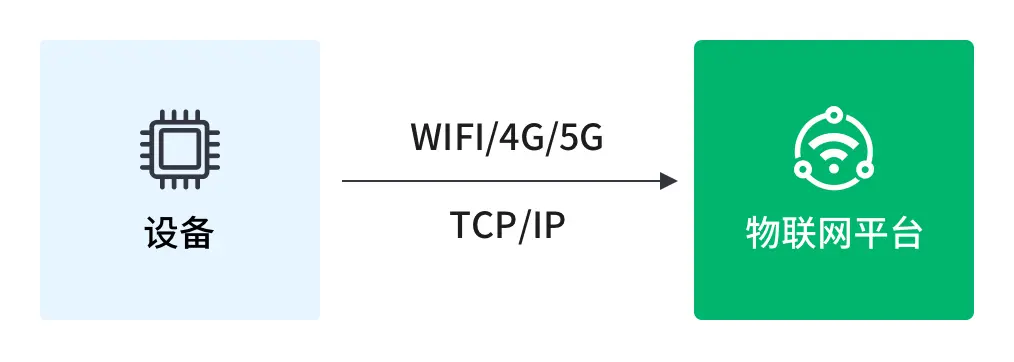
\includegraphics[width=0.8\linewidth]{../design/IoT1.png}
    \caption{IoT1}
    \label{fig:IoT1}
\end{figure}

网关协议是适用于短距通信无法直接上云的协议,比如蓝牙、ZigBee、LoRa 等。此类设备需要接入网关转换之后,通过 TCP/IP 协议进行上云。

\begin{figure}[H]
    \centering
    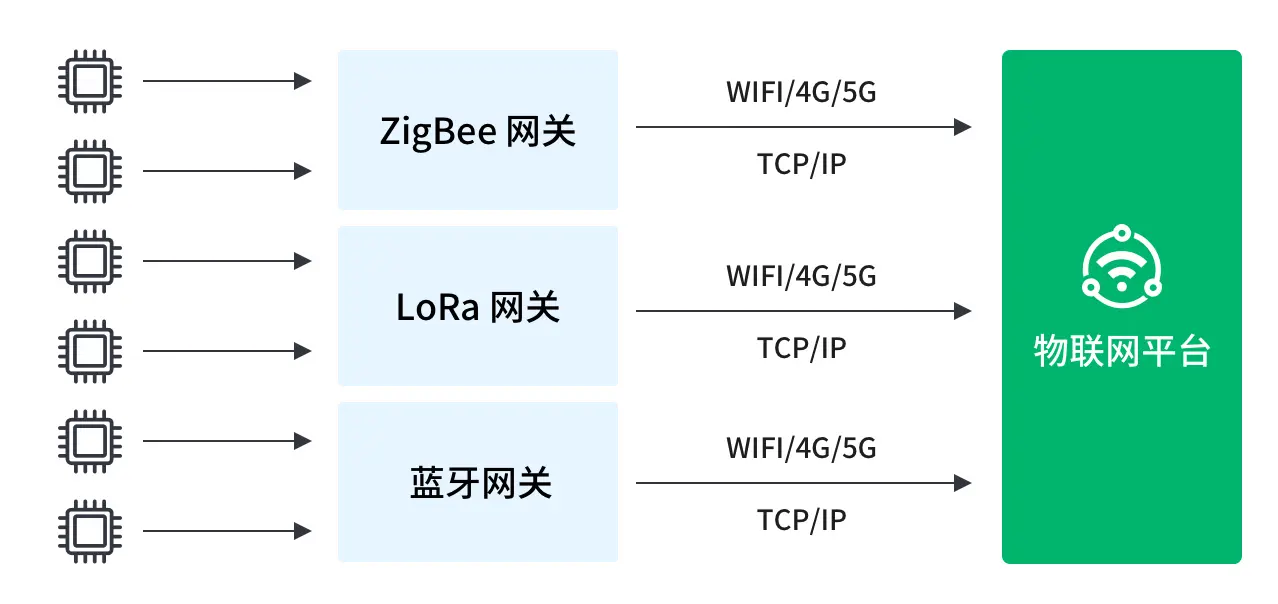
\includegraphics[width=0.8\linewidth]{../design/IoT2.png}
    \caption{IoT2}
    \label{fig:IoT2}
\end{figure}

本系统不考虑网关协议,只考虑应用层协议。系统将支持不同种类的电子秤,支持包含 HTTP、MQTT、MQTT-SN、CoAP、STOMP 在内的多种物联网通信协议。

为了降低开发成本,除了 HTTP、MQTT 这两种通信协议,其它物联网协议采用网关转换的方法来提供支持,网关将对各类协议转换成 MQTT 协议与 MQTT Broker 进行通信,认证规则和消息的持久化规则遵循 MQTT 协议标准。

下面对通信协议进行分析。

这里主要分析两种协议:HTTP 和 MQTT。

HTTP(HyperText Transfer Protocol)即超文本传输协议,是一种用于分布式、协作式和超媒体信息系统的应用层协议。在电子秤系统中,通过调用 HTTP 接口上传称重信息具有以下特点:

一、稳定性和通用性:HTTP 是互联网上广泛使用的协议,具有很高的稳定性和通用性。几乎所有的网络设备和软件都支持 HTTP 协议,这使得电子秤可以很容易地与各种不同的系统进行集成。无论是传统的服务器架构,还是现代的云服务平台,都可以通过 HTTP 接口接收电子秤上传的称重信息。例如,许多企业的内部管理系统、电商平台的库存管理系统等都可以通过 HTTP 接口与电子秤进行数据交互,实现实时的库存更新和物流跟踪\cite{Zhao2016}。

二、易于开发和调试:HTTP 协议的开发和调试工具非常丰富。开发人员可以使用常见的编程语言和开发框架,如 Java、Python、Node.js 等,轻松地实现 HTTP 接口的调用和数据处理。同时,各种网络调试工具,如 Postman、Fiddler 等,可以帮助开发人员快速地测试和调试电子秤与服务器之间的通信,确保数据的准确传输。

三、支持多种数据格式:HTTP 协议支持多种数据格式的传输,如 JSON、XML 等。这使得电子秤可以根据不同的应用需求,选择合适的数据格式上传称重信息。例如,对于需要与第三方系统进行数据集成的场景,可以选择使用 JSON 格式,因为 JSON 格式具有简洁、易读、易于解析等优点,被广泛应用于 Web 开发和数据交换领域。

MQTT(Message Queuing Telemetry Transport)即消息队列遥测传输协议,是一种轻量级的发布/订阅模式的消息传输协议。在电子秤系统中,发送 MQTT 消息上传称重信息具有以下优势:

一、低带宽和低功耗:MQTT 协议非常适合在低带宽和低功耗的环境下使用。对于电子秤等物联网设备来说,通常需要在有限的网络资源和电池电量下进行数据传输。MQTT 协议通过采用轻量级的消息格式和高效的发布/订阅模式,可以大大降低网络带宽的占用和设备的功耗。例如,在一些偏远地区或者移动环境下,网络带宽可能非常有限,此时使用 MQTT 协议可以确保电子秤能够及时上传称重信息,同时不会对网络造成过大的负担\cite{Jia2015}。

二、实时性和可靠性:MQTT 协议支持 QoS(Quality of Service)级别,可以根据不同的应用需求,选择不同的消息传输质量级别。在 MQTT 协议中,QoS 有三种级别\cite{Jia2015},分别是:
\begin{itemize}
    \item QoS0 – “最多一次”:消息最多传送一次,不保证消息到达目标。适用于实时性要求非常高,但对消息丢失容忍的场景。
    \item QoS1 – “至少一次”:保证消息至少传送一次,但可能会重复。适用于需要消息可靠到达,但不介意重复接收的情况。
    \item QoS2 – “只有一次”:确保每条消息只会传送一次,且无重复。适用于对消息的唯一性和可靠性有较高要求的场景。
\end{itemize}

对于需要实时上传称重信息的场景,可以选择 QoS1 或 QoS2 级别,确保消息的可靠传输。同时,MQTT 协议的发布/订阅模式可以实现实时的数据推送,当电子秤上传称重信息后,订阅了该主题的客户端可以立即收到消息,实现实时的数据更新。

三、易于扩展和集成:MQTT 协议具有良好的扩展性和集成性。可以很容易地与其他物联网协议和技术进行集成,如 CoAP、HTTP、WebSocket 等。同时,MQTT 协议的发布/订阅模式可以支持大规模的设备连接和数据传输,适用于构建物联网应用平台。例如,在智慧农业大棚测控系统中,采用 MQTT 协议将智慧大棚测控系统和阿里云物联网平台结合在一起,通过手机 APP 或 PC 软件访问阿里云服务器数据库,实现了移动终端对农业大棚实时监测和控制\cite{Liang2020}。

\subsubsection{服务接口设计}

本系统服务接口包含四个部分,分别是用户管理模块、果实模块、工作服务模块和称重服务模块。具体接口功能和路径设计如表格\ref{tab:用户管理模块接口设计}、表格\ref{tab:果实模块接口设计}、表格\ref{tab:工作服务模块接口设计}和表格\ref{tab:工作服务模块接口设计}所示。

% 用户管理模块表格
\begin{table}[H]
\centering
% \resizebox{\textwidth}{!}{%
\begin{tabular}{|c|c|c|}
\hline
\textbf{接口名称} & \textbf{HTTP方法} & \textbf{接口路径} \\
\hline
用户登录 & POST & /user/login \\
\hline
获取个人信息 & GET & /user \\
\hline
更新个人信息 & PUT & /user/me \\
\hline
获取用户列表 & GET & /user/list \\
\hline
获取用户信息 & GET & /user/{uid} \\
\hline
添加用户 & POST & /user \\
\hline
更新用户 & PUT & /user \\
\hline
\end{tabular}%

    % }
\caption{用户管理模块接口设计}
\label{tab:用户管理模块接口设计}
\end{table}

% 果实模块表格
\begin{table}[H]
\centering
% \resizebox{\textwidth}{!}{%
\begin{tabular}{|c|c|c|}
\hline
\textbf{接口名称} & \textbf{HTTP方法} & \textbf{接口路径} \\
\hline
获取果实列表 & GET & /produce/list \\
\hline
获取果实 & GET & /produce/{id} \\
\hline
根据名称获取果实 & GET & /produce \\
\hline
添加果实 & POST & /produce \\
\hline
更新果实 & PUT & /produce \\
\hline
获取果实年产量 & GET & /produce/summary/year \\
\hline
获取果实分批产量 & GET & /produce/summary/work \\
\hline
\end{tabular}%

% }
\caption{果实模块接口设计}
\label{tab:果实模块接口设计}
\end{table}

% 工作服务模块表格
\begin{table}[H]
\centering
% \resizebox{\textwidth}{!}{%
\begin{tabular}{|c|c|c|}
\hline
\textbf{接口名称} & \textbf{HTTP方法} & \textbf{接口路径} \\
\hline
获取采摘工作列表 & GET & /work/list \\
\hline
获取采摘工作 & GET & /work/{id} \\
\hline
获取果实的采摘工作列表 & GET & /work/produce/{id} \\
\hline
添加采摘工作 & POST & /work \\
\hline
更新采摘工作 & PUT & /work \\
\hline
获取采摘作业的分配情况 & GET & /work/{id}/assignments \\
\hline
获取我被分配的工作 & GET & /work/assignments/me \\
\hline
分配工作 & POST & /work/assign \\
\hline
重新分配工作 & PUT & /work/assign \\
\hline
\end{tabular}%

% }
\caption{工作服务模块接口设计}
\label{tab:工作服务模块接口设计}
\end{table}

% 称重服务模块表格
\begin{table}[H]
\centering
% \resizebox{\textwidth}{!}{%
\begin{tabular}{|c|c|c|}
\hline
\textbf{接口名称} & \textbf{HTTP方法} & \textbf{接口路径} \\
\hline
获取电子秤列表 & GET & /weigh/scale/list \\
\hline
获取电子秤 & GET & /weigh/scale/{id} \\
\hline
根据key获取电子秤 & GET & /weigh/scale \\
\hline
添加电子秤 & POST & /weigh/scale \\
\hline
更新电子秤信息 & PUT & /weigh/scale \\
\hline
添加称重记录 & POST & /weigh/record \\
\hline
获取称重记录 & POST & /weigh/record/list \\
\hline
获取员工各作业采摘量 & GET & /weigh/summary \\
\hline
\end{tabular}%

% }
\caption{称重服务模块接口设计}
\label{tab:称重服务模块接口设计}
\end{table}

\subsubsection{数据库设计}

本软件数据库设计分为三个阶段:概念模型设计、逻辑模型设计和物理模型设计,下面进行具体阐述。

首先,进行概念模型设计:

农业果实称重云端软件中,可以抽象出七个实体对象,分别是果实、员工、电子秤、采摘作业、称重记录、MQTT客户端、MQTT授权信息,具体分析如下:

\begin{itemize}
    \item 果实(Fruit):代表农场中的果实,具有编号(ID)属性。
    \item 员工(Employee):代表农场中的员工,具有编号(ID)属性。
    \item 电子秤(Electronic Scale):代表用于称重果实的电子秤,具有编号(ID)和密钥(Key)属性。
    \item MQTT 客户端(MQTT Client):代表用于连接 MQTT 服务器的客户端,具有编号(ID)和密码(Password)属性。
    \item 采摘作业(Picking Task):代表员工采摘果实的作业,具有开始时间、结束时间和采摘结果属性。
    \item 称重记录(Weighing Record):代表电子秤记录的果实重量,具有称重结果和称重时间属性。
    \item MQTT 授权信息(MQTT Authorization Info):代表 MQTT 客户端的授权信息,具有权限信息属性。
\end{itemize}

针对上述对象,根据实际的业务场景,可以得到如下关系:

\begin{table}[H]
\centering
\resizebox{\textwidth}{!}{%
\begin{tabular}{|c|c|c|c|}
\hline
\textbf{关系名称} & \textbf{关系类型} & \textbf{描述} \\
\hline
果实 - 采摘关系 & 一对多(1:N) & 一个果实可以被多次采摘,与多个采摘作业相关联。 \\
\hline
员工 - 员工称重记录 & 一对多(1:N) & 一个员工可以进行多次称重记录。  \\
\hline
员工 - 采摘作业 & 一对多(1:N) & 一个员工可以执行多个采摘作业。  \\
\hline
电子秤 - 电子秤称重记录 & 一对多(1:N) & 一个电子秤可以记录多个称重记录。  \\
\hline
电子秤 - 称重记录 & 一对多(1:N) & 一个电子秤可以记录多个称重记录。\\
\hline
采摘作业 - 称重记录 & 一对多(1:N) & 一个采摘作业可以产生多个称重记录(例如,在不同时间多次称重)。  \\
\hline
MQTT 客户端 - 设备认证 & 一对一(1:1) & 每个 MQTT 客户端都必须进行设备认证。 \\
\hline
MQTT 客户端 - 设备授权 & 一对多(1:N) & 一个 MQTT 客户端可以拥有多个授权信息。  \\
\hline
员工 - 称重记录 & 一对多(1:N) & 一个员工可以产生多个称重记录。\\
\hline
电子秤 - 设备认证 & 一对一(1:1) & 每个电子秤都必须进行设备认证。  \\
\hline
\end{tabular}%
}
\caption{实体关系及属性表}
\end{table}

将上述分析进行归纳,得到 ER 图如下:

\begin{figure}[H]
    \centering
    \includegraphics[width=0.8\linewidth]{../design/out/数据库设计-ER.png}
    \caption{数据库设计-ER}
    \label{fig:数据库设计-ER}
\end{figure}

该 ER 图展示了一个农场管理系统中各个实体之间的复杂关系,包括果实、员工、电子秤和 MQTT 客户端。通过这些关系,系统可以有效地跟踪果实的采摘、称重和授权信息,从而实现高效的农场管理。

完成概念模型设计,可以开始进行逻辑模型设计:

本部分详细描述了系统各个表的结构及其字段定义,涵盖了表之间的关系、字段的数据类型及约束条件。每个表的设计都遵循规范化原则,以确保数据的一致性、完整性和高效性。字段的定义包括主键、外键、唯一约束、非空约束等,同时考虑了查询和更新的效率,力求在保证系统扩展性的同时,实现良好的性能表现。

% t_produce table
\begin{table}[H]
    \centering
    \caption{产品表 (t\_produce)}
    \begin{tabular}{|l|l|l|l|}
        \hline
        \textbf{字段} & \textbf{类型} & \textbf{可空} & \textbf{说明} \\
        \hline
        id & BIGINT & 否 & 主键,自增 \\
        name & VARCHAR(255) & 是 & 产品名称 \\
        type & INT & 是 & 产品类型 \\
        create\_time & BIGINT & 否 & 创建时间 \\
        update\_time & BIGINT & 否 & 更新时间 \\
        status & INT & 否 & 状态 \\
        \hline
    \end{tabular}
\end{table}

% t_record table
\begin{table}[H]
    \centering
    \caption{记录表 (t\_record)}
    \begin{tabular}{|l|l|l|l|}
        \hline
        \textbf{字段} & \textbf{类型} & \textbf{可空} & \textbf{说明} \\
        \hline
        id & BIGINT & 否 & 主键,自增 \\
        work\_id & BIGINT & 否 & 工作ID \\
        employee\_id & BIGINT & 否 & 员工ID \\
        scale\_id & BIGINT & 否 & 秤ID \\
        data\_value & DECIMAL(10,2) & 是 & 数据值 \\
        data\_error\_margin & DECIMAL(10,2) & 是 & 误差范围 \\
        unit & INT & 否 & 单位 \\
        data\_time & BIGINT & 否 & 数据时间 \\
        \hline
    \end{tabular}
\end{table}

% t_scale table
\begin{table}[H]
    \centering
    \caption{秤表 (t\_scale)}
    \begin{tabular}{|l|l|l|l|}
        \hline
        \textbf{字段} & \textbf{类型} & \textbf{可空} & \textbf{说明} \\
        \hline
        id & BIGINT & 否 & 主键,自增 \\
        skey & VARCHAR(255) & 是 & 秤标识 \\
        model & VARCHAR(255) & 是 & 型号 \\
        max\_capacity & DECIMAL(10,2) & 是 & 最大容量 \\
        min\_capacity & DECIMAL(10,2) & 是 & 最小容量 \\
        unit & INT & 否 & 单位 \\
        verification\_interval & INT & 否 & 检定间隔 \\
        display\_interval & INT & 否 & 显示间隔 \\
        unit\_dv & INT & 否 & 分度值单位 \\
        protocol & INT & 否 & 协议 \\
        create\_time & BIGINT & 否 & 创建时间 \\
        update\_time & BIGINT & 否 & 更新时间 \\
        status & INT & 否 & 状态 \\
        \hline
    \end{tabular}
\end{table}

% t_user table
\begin{table}[H]
    \centering
    \caption{用户表 (t\_user)}
    \begin{tabular}{|l|l|l|l|}
        \hline
        \textbf{字段} & \textbf{类型} & \textbf{可空} & \textbf{说明} \\
        \hline
        id & BIGINT & 否 & 主键,自增 \\
        uid & VARCHAR(255) & 是 & 用户ID \\
        cid & VARCHAR(255) & 是 & 客户ID \\
        name & VARCHAR(255) & 是 & 用户名 \\
        password & VARCHAR(255) & 是 & 密码 \\
        roles & VARCHAR(255) & 是 & 角色 \\
        create\_time & BIGINT & 否 & 创建时间 \\
        update\_time & BIGINT & 否 & 更新时间 \\
        status & INT & 否 & 状态 \\
        \hline
    \end{tabular}
\end{table}

% t_work table
\begin{table}[H]
    \centering
    \caption{工作表 (t\_work)}
    \begin{tabular}{|l|l|l|l|}
        \hline
        \textbf{字段} & \textbf{类型} & \textbf{可空} & \textbf{说明} \\
        \hline
        id & BIGINT & 否 & 主键,自增 \\
        produce\_id & BIGINT & 否 & 产品ID \\
        start\_time & BIGINT & 否 & 开始时间 \\
        end\_time & BIGINT & 否 & 结束时间 \\
        data\_value & DECIMAL(10,2) & 是 & 数据值 \\
        unit & INT & 否 & 单位 \\
        create\_time & BIGINT & 否 & 创建时间 \\
        update\_time & BIGINT & 否 & 更新时间 \\
        status & INT & 否 & 状态 \\
        \hline
    \end{tabular}
\end{table}

% t_mqtt_user table
\begin{table}[H]
    \centering
    \caption{MQTT用户表 (t\_mqtt\_user)}
    \begin{tabular}{|l|l|l|l|}
        \hline
        \textbf{字段} & \textbf{类型} & \textbf{可空} & \textbf{说明} \\
        \hline
        id & INT & 否 & 主键,自增 \\
        username & VARCHAR(100) & 是 & 用户名 \\
        password\_hash & VARCHAR(100) & 是 & 密码哈希 \\
        salt & VARCHAR(35) & 是 & 盐值 \\
        is\_superuser & TINYINT(1) & 是 & 是否超级用户 \\
        created & DATETIME & 是 & 创建时间 \\
        \hline
    \end{tabular}
\end{table}

% t_mqtt_acl table
\begin{table}[H]
    \centering
    \caption{MQTT访问控制表 (t\_mqtt\_acl)}
    \begin{tabular}{|l|l|l|l|}
        \hline
        \textbf{字段} & \textbf{类型} & \textbf{可空} & \textbf{说明} \\
        \hline
        id & INT & 否 & 主键,自增 \\
        username & VARCHAR(100) & 否 & 用户名 \\
        permission & VARCHAR(5) & 否 & 权限(allow/deny) \\
        action & VARCHAR(9) & 否 & 操作类型 \\
        topic & VARCHAR(100) & 否 & 主题 \\
        qos & TINYINT(1) & 是 & QoS等级 \\
        retain & TINYINT(1) & 是 & 是否保留消息 \\
        \hline
    \end{tabular}
\end{table}

最后,完成物理模型设计:

本系统使用 MySQL 作为数据库管理系统,采用 InnoDB 存储引擎,事务隔离级别设置为可重复读,以确保数据的一致性和可靠性。在后台应用中,数据库访问通过 JPA (Java Persistence API) 进行实现,简化了数据库操作,提升了代码的可维护性和开发效率。

\subsection{系统功能实现}
\subsubsection{登录界面}

启动前后台服务,访问 8081 端口,即可进入登录界面:

\begin{figure}[H]
    \centering
    
\includegraphics[width=0.8\linewidth]{../result/登录界面.png}
    \caption{登录界面}
    \label{fig:登录界面}
\end{figure}

用户可以通过用户唯一编号(身份证)和密码完成登录。

\subsubsection{个人信息模块}

在登录界面完成登录后,即可进入个人中心:

\begin{figure}[H]
    \centering
    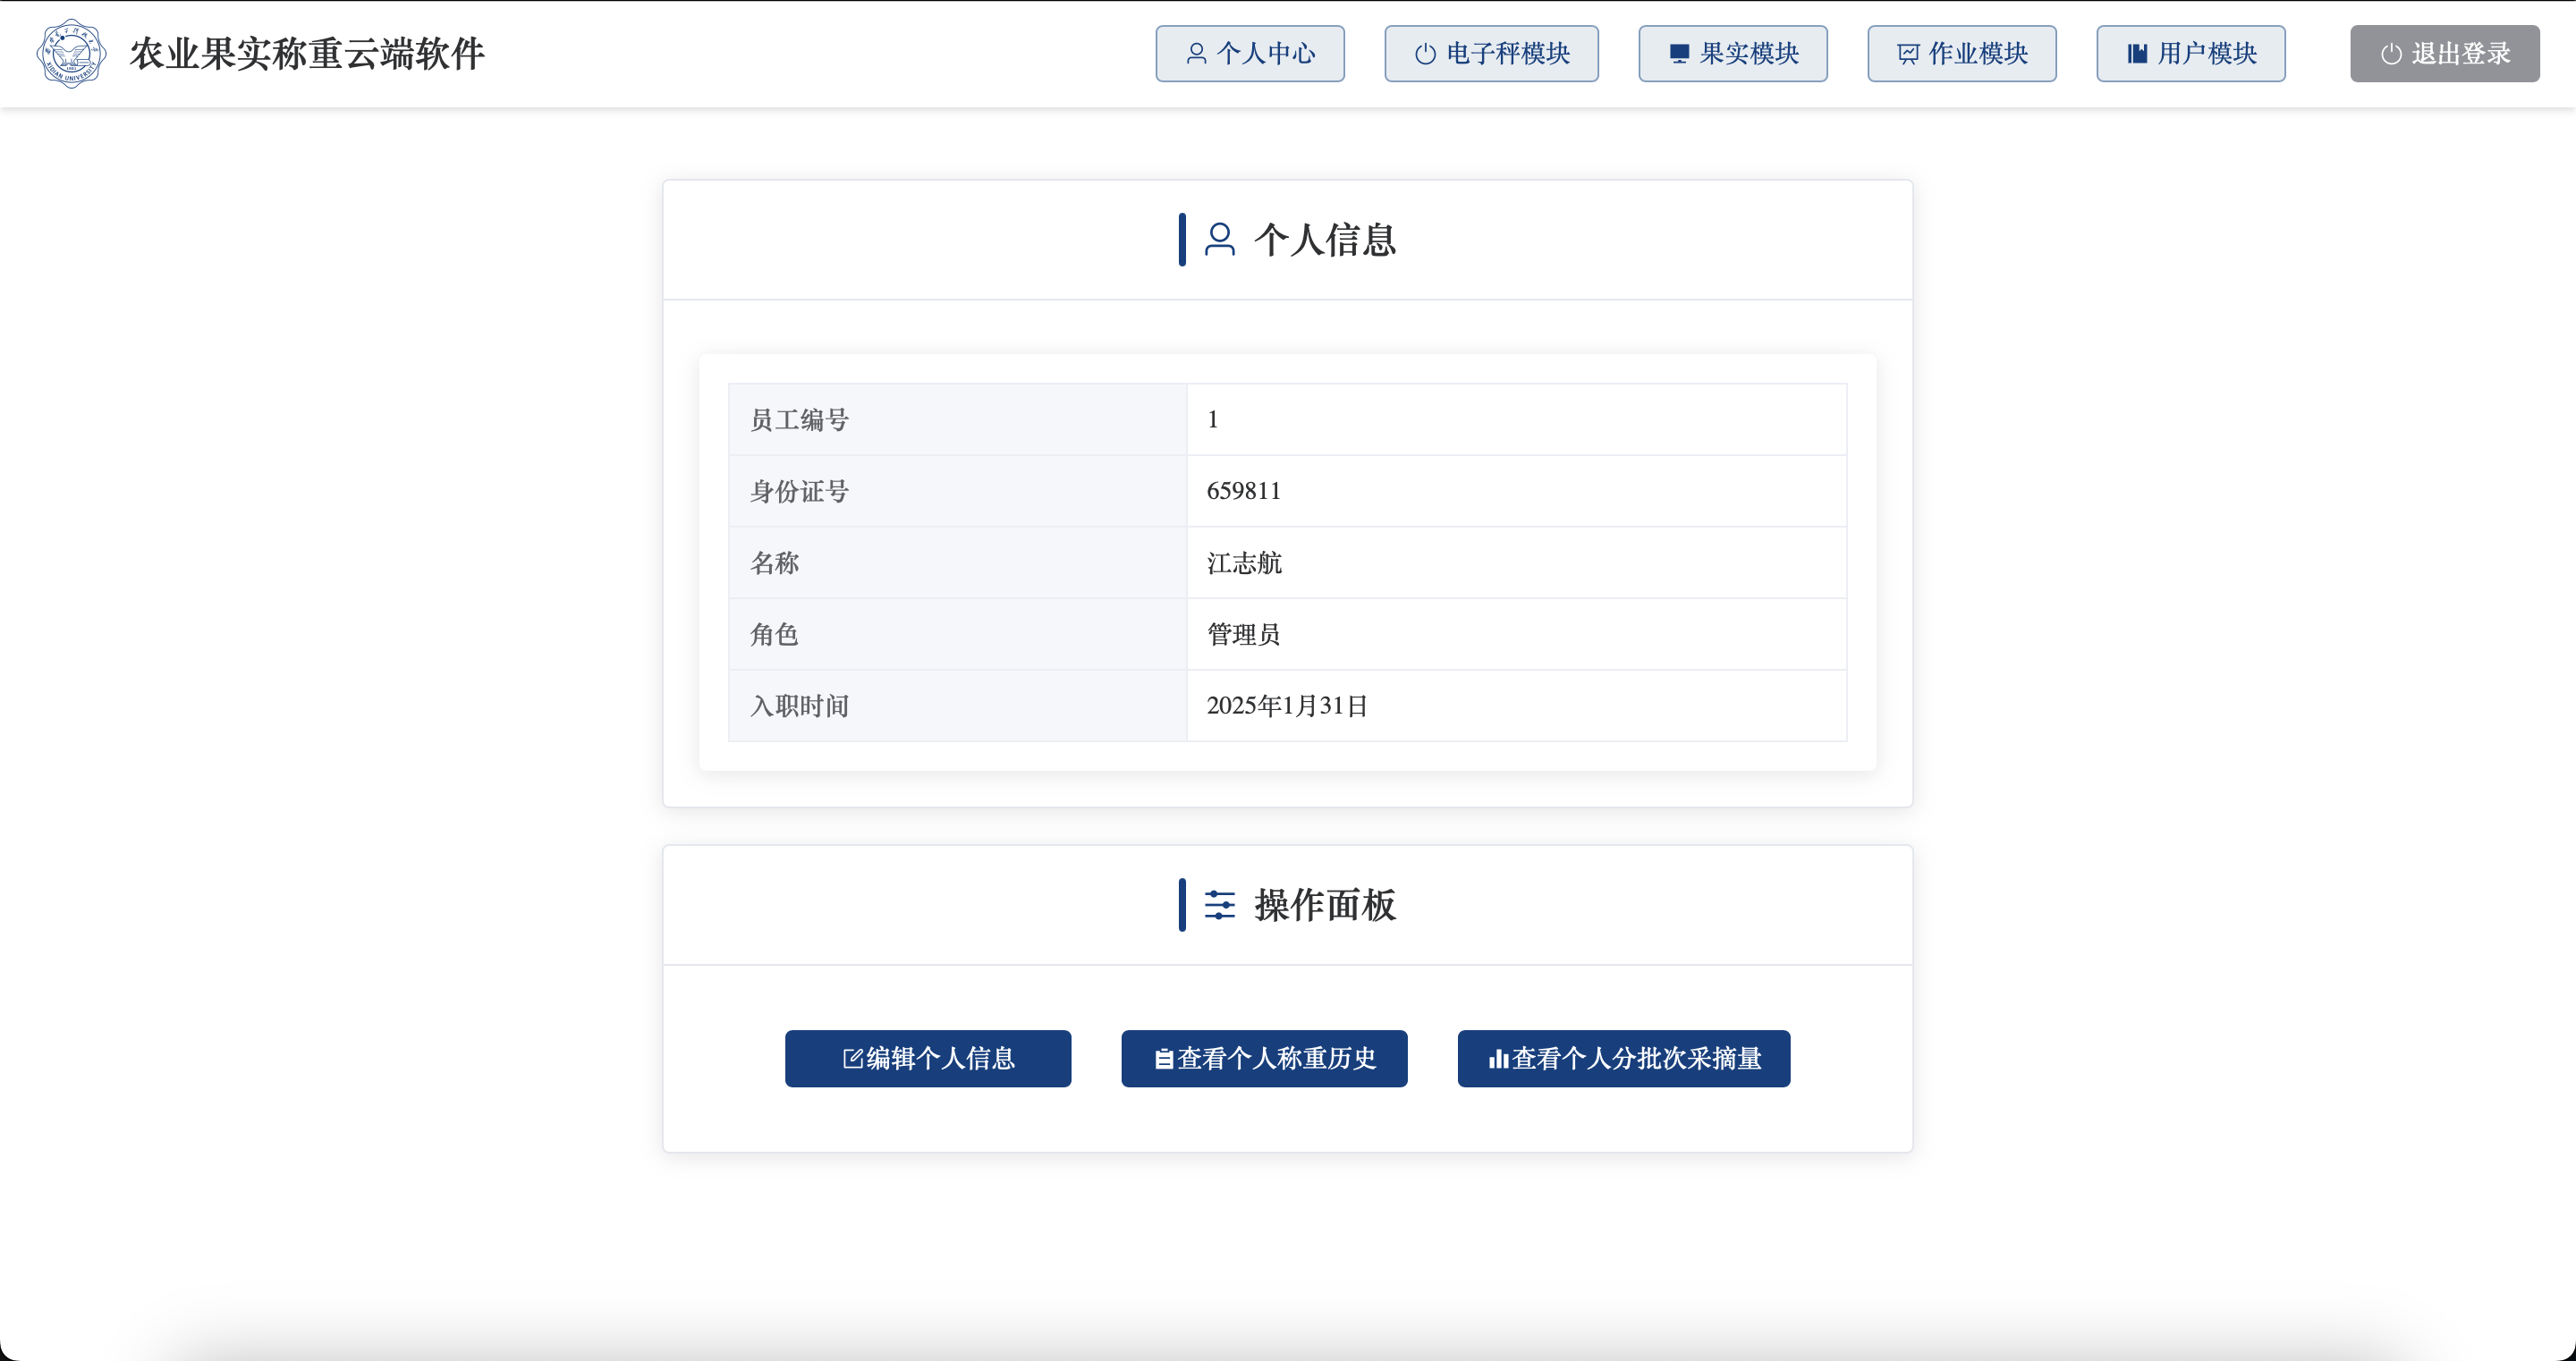
\includegraphics[width=0.8\linewidth]{../result/个人中心.png}
    \caption{个人中心}
    \label{fig:个人中心}
\end{figure}

在个人中心,用户可以查看或更新个人信息。

用户可以点击查看个人称重历史:

\begin{figure}[H]
    \centering
    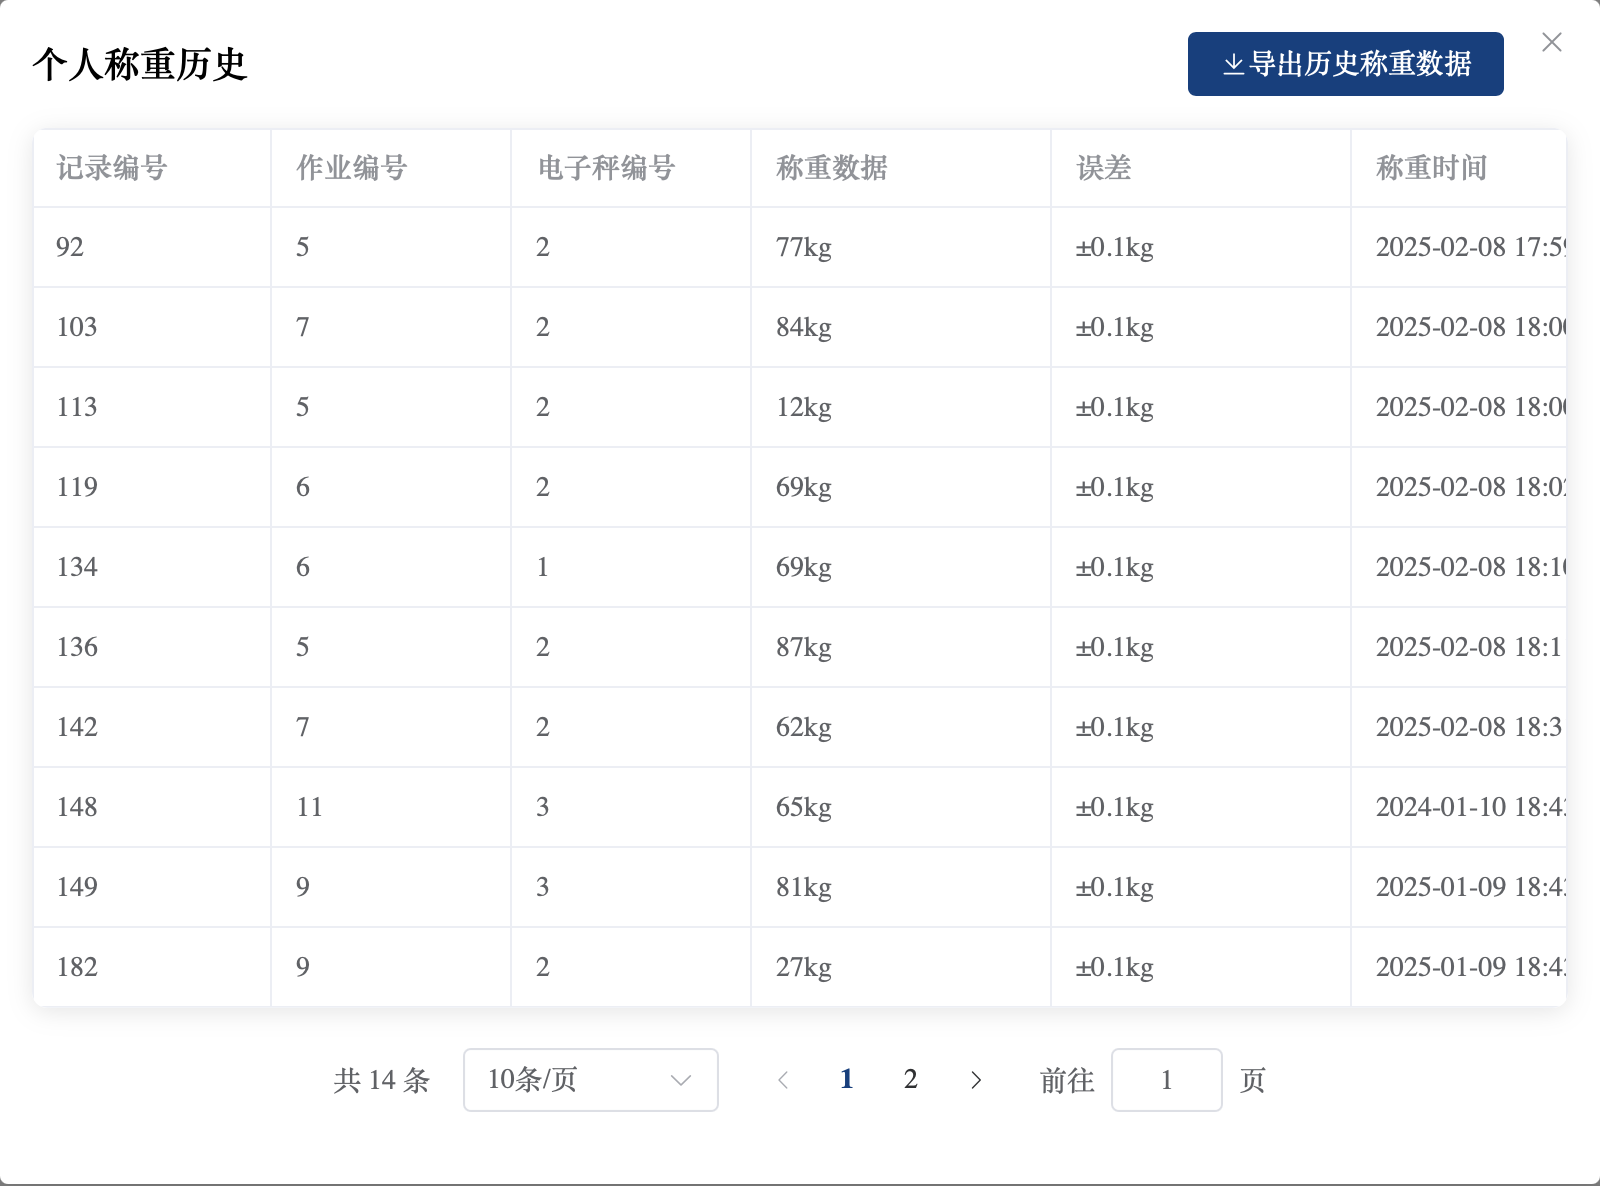
\includegraphics[width=0.8\linewidth]{../result/个人称重历史.png}
    \caption{个人称重历史}
    \label{fig:个人称重历史}
\end{figure}

用户可以点击查看个人分批次采摘量:

\begin{figure}[H]
    \centering
    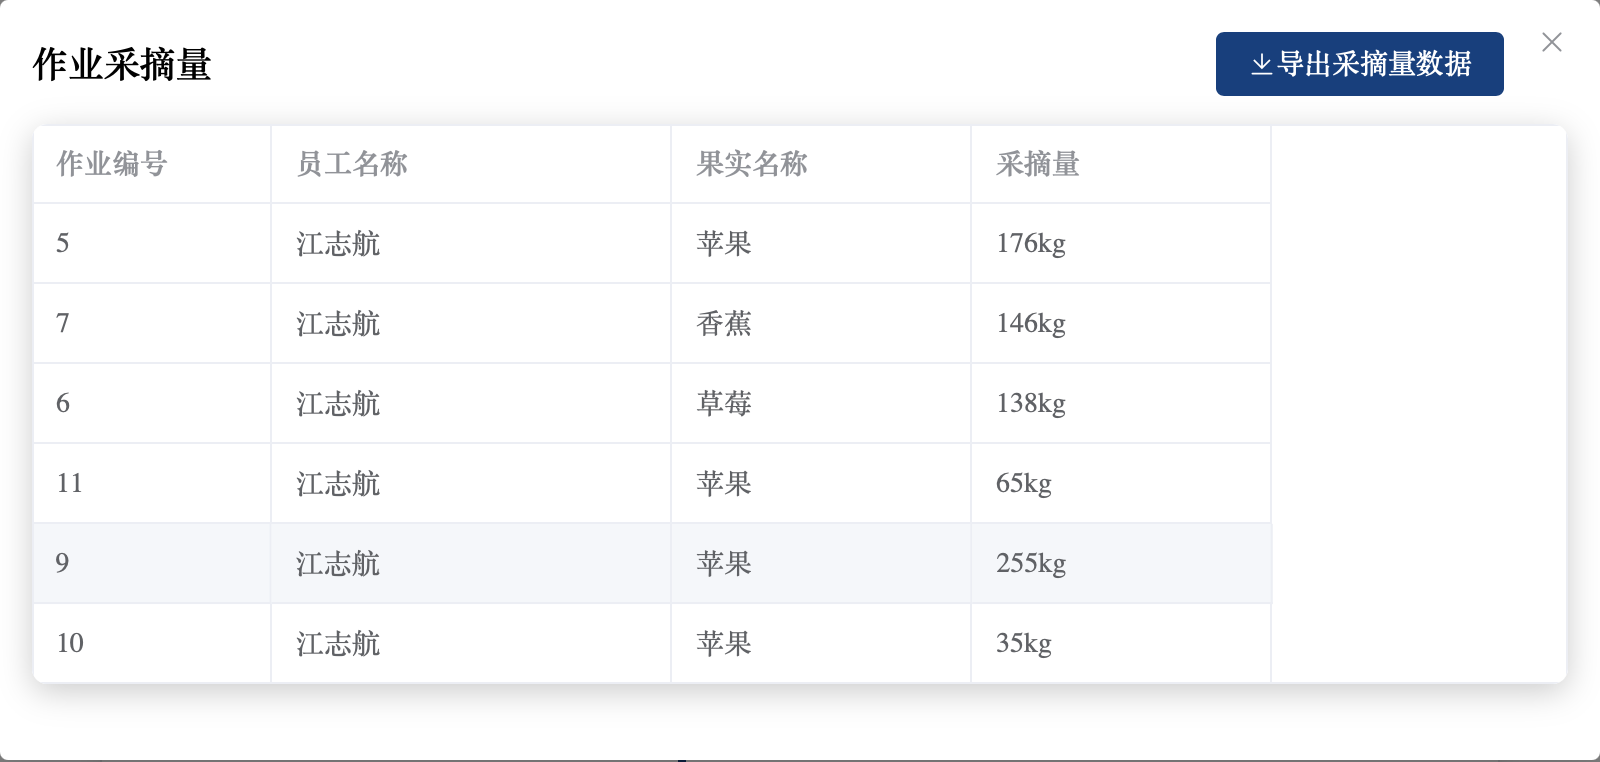
\includegraphics[width=0.8\linewidth]{../result/个人分批次采摘量.png}
    \caption{个人分批次采摘量}
    \label{fig:个人分批次采摘量}
\end{figure}

\subsubsection{工作服务模块}

在上方导航处,点击作业模块,进入作业模块界面:

\begin{figure}[H]
    \centering
    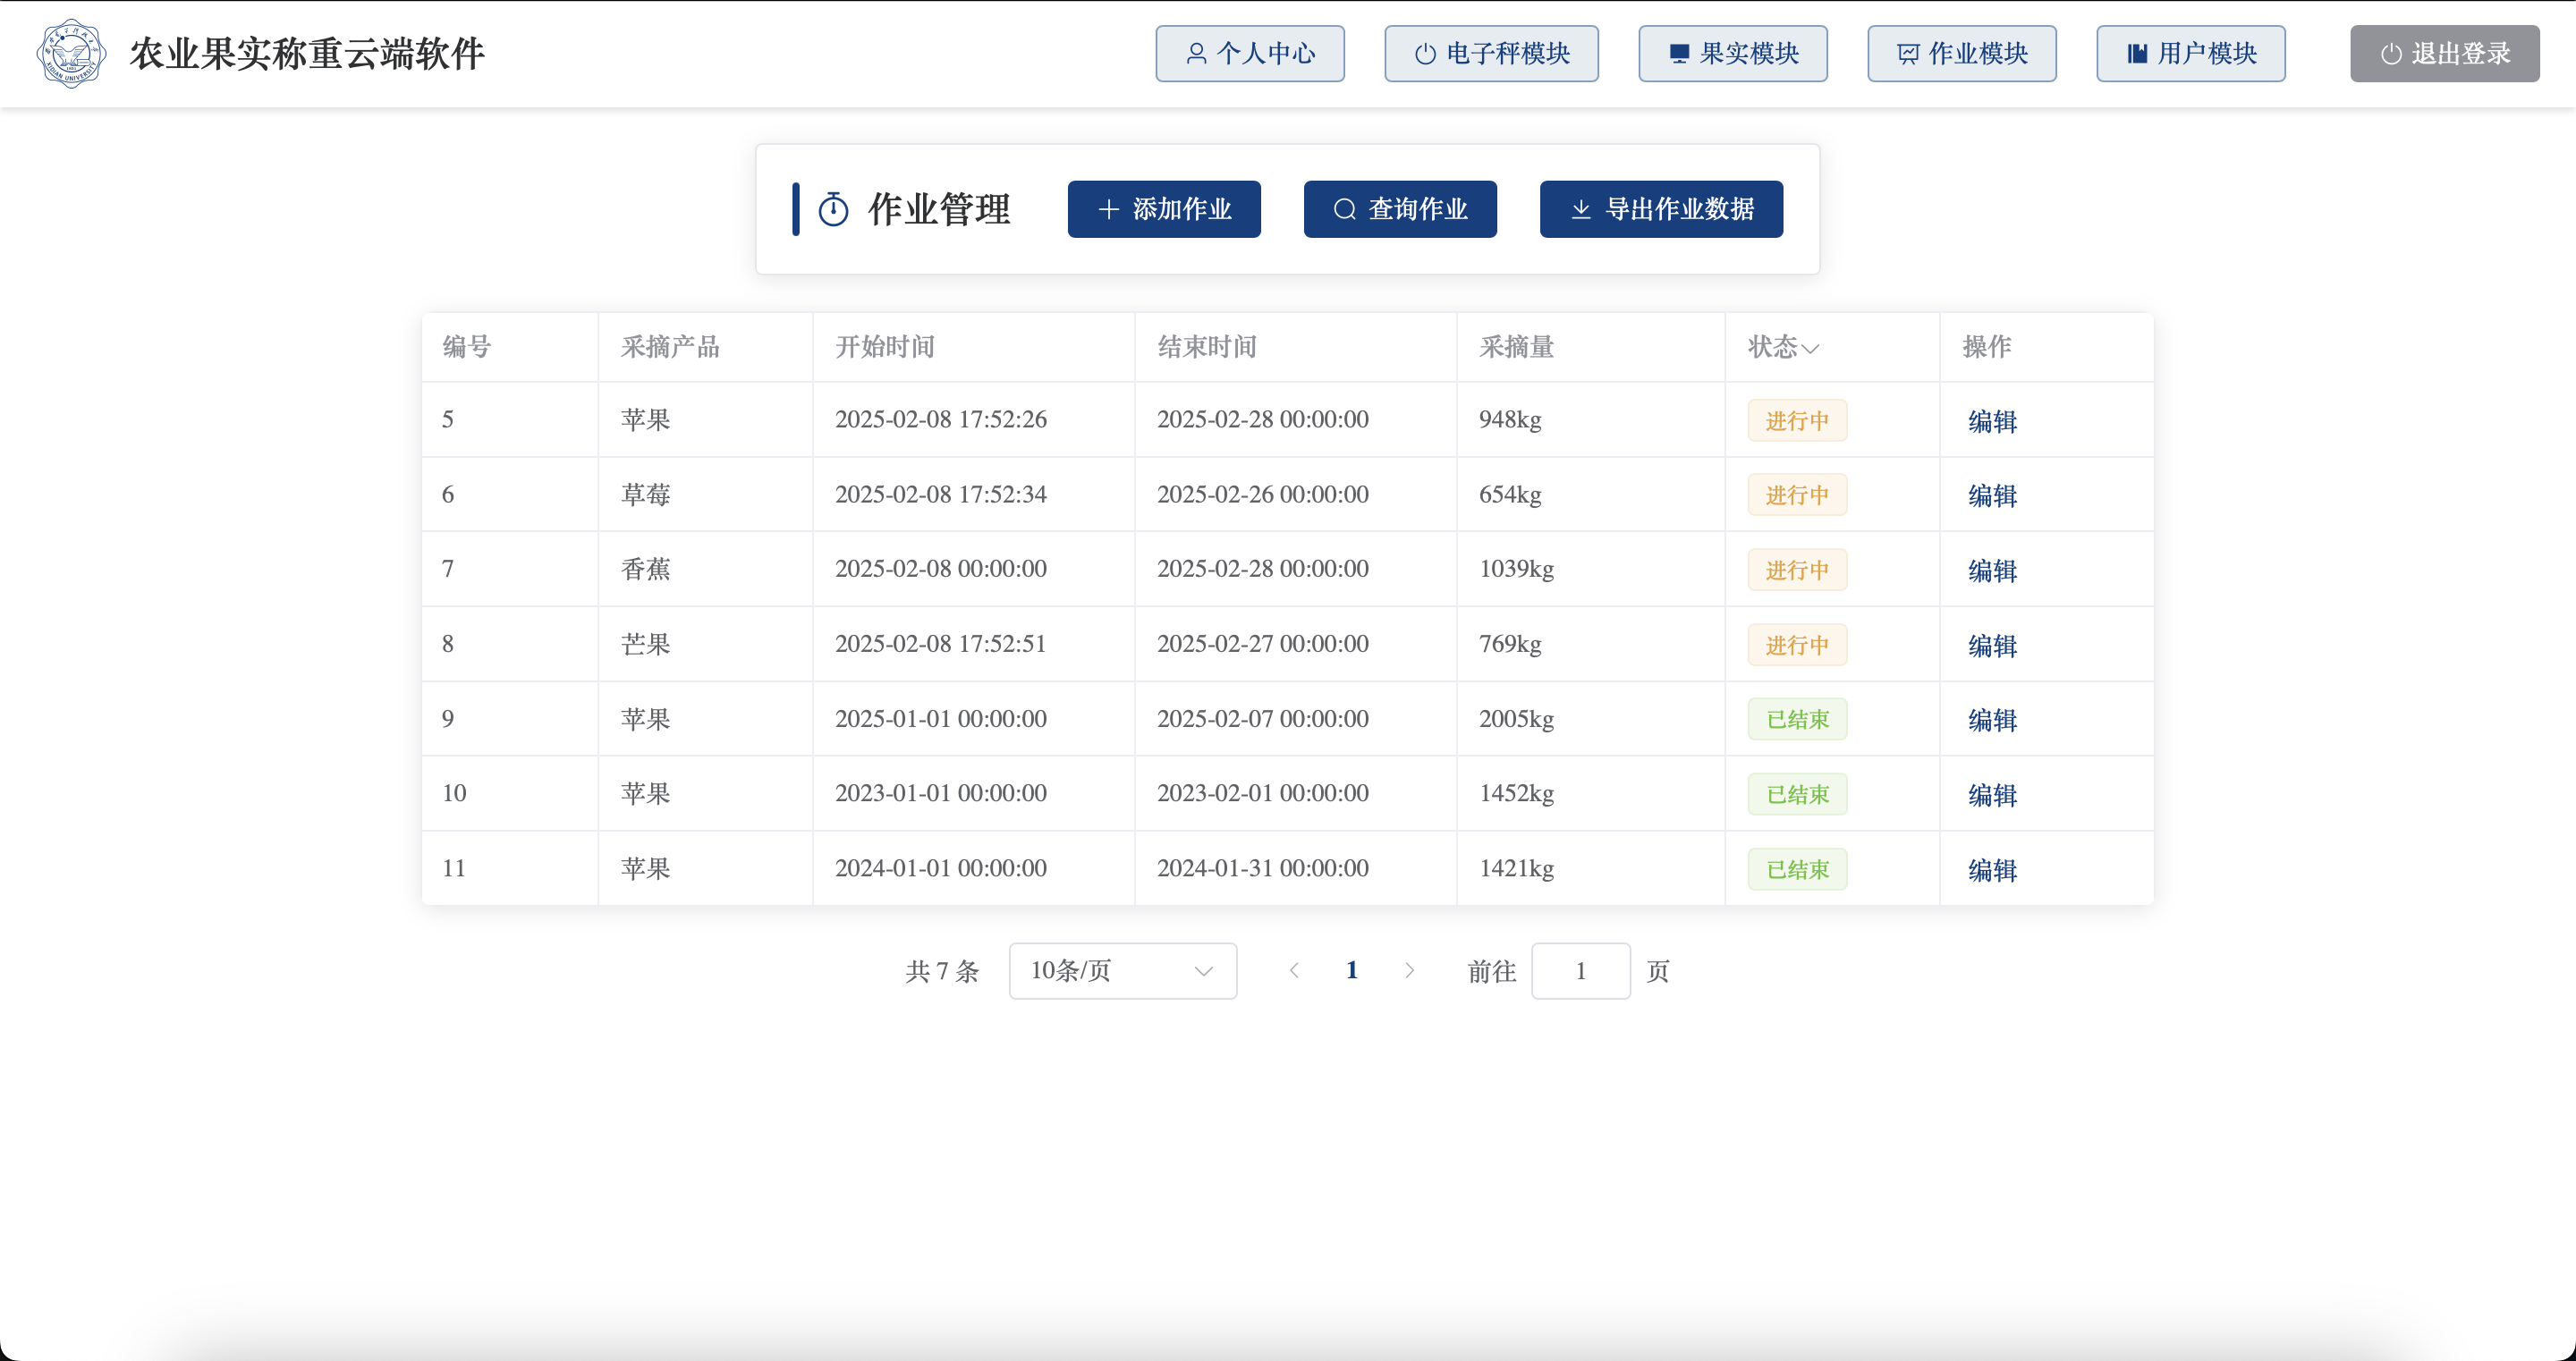
\includegraphics[width=0.8\linewidth]{../result/作业模块.png}
    \caption{作业模块}
    \label{fig:作业模块}
\end{figure}

在作业模块中,目前支持对作业执行查看、新增、更新、查询和导出数据等操作。

\subsubsection{称重服务模块}

在上方导航处,点击电子秤模块,进入电子秤模块界面:

\begin{figure}[H]
    \centering
    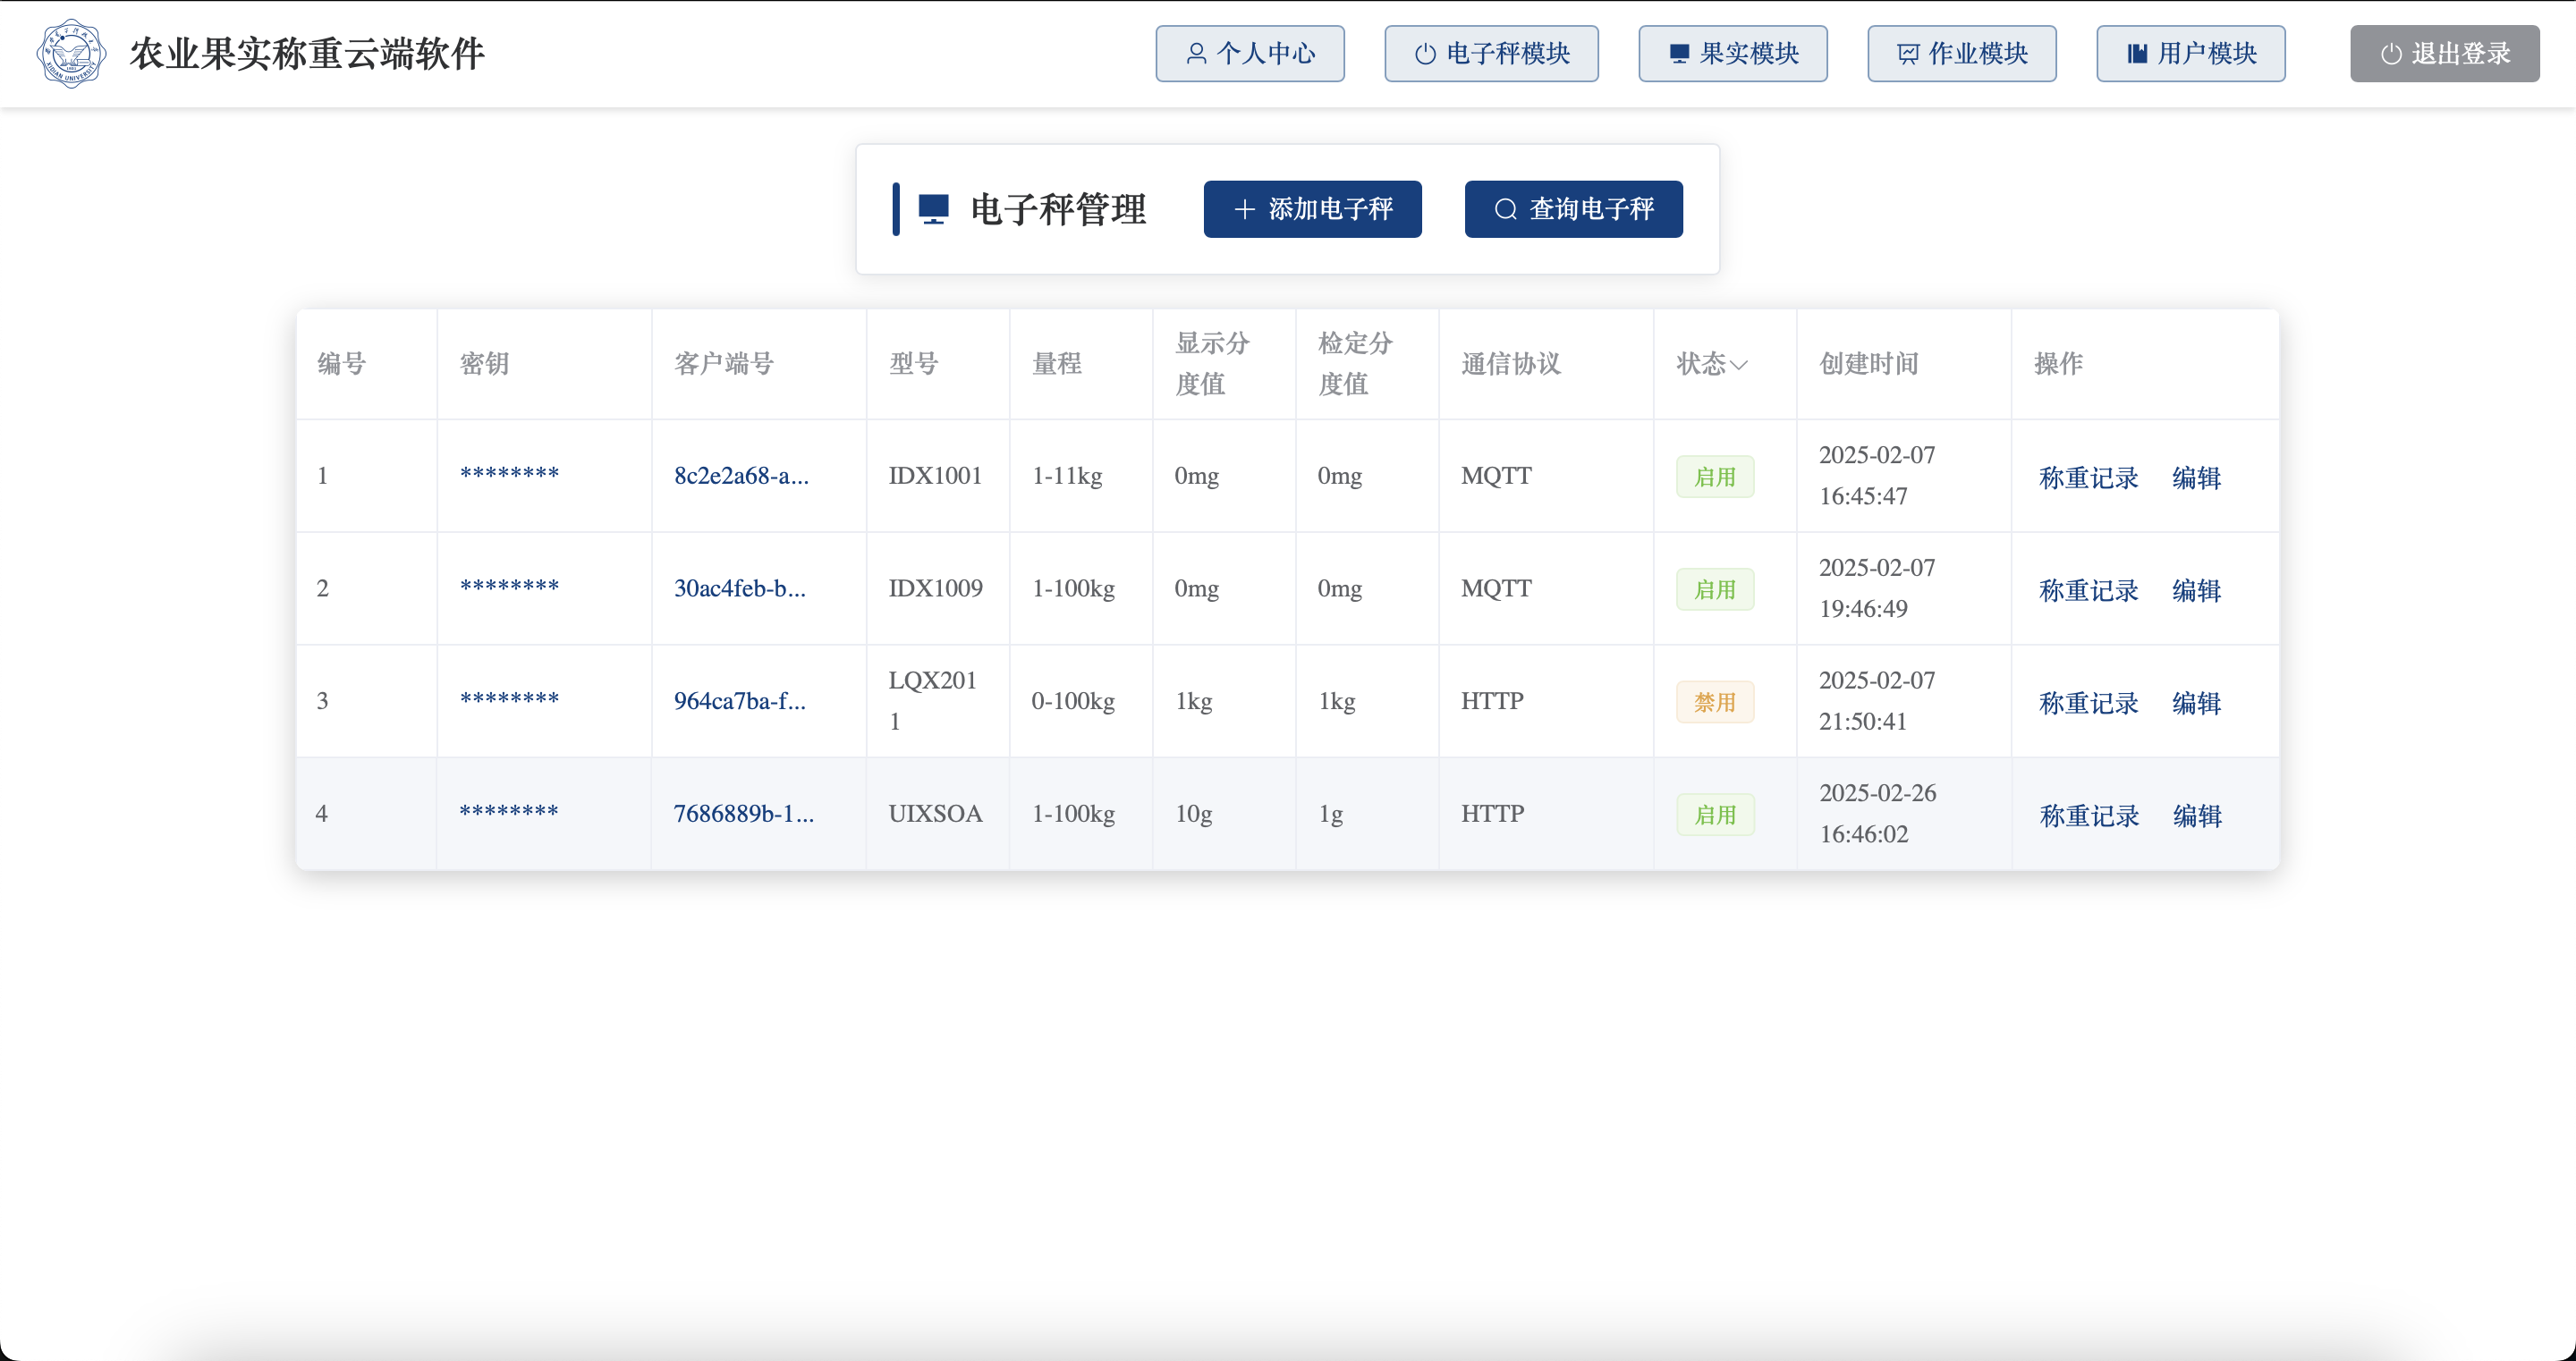
\includegraphics[width=0.8\linewidth]{../result/电子秤模块.png}
    \caption{电子秤模块}
    \label{fig:电子秤模块}
\end{figure}

在该界面中,用户可以查看、新增、查询和更新电子秤。

在任一电子秤中,用户可以点击称重记录按钮查看称重记录:

\begin{figure}[H]
    \centering
    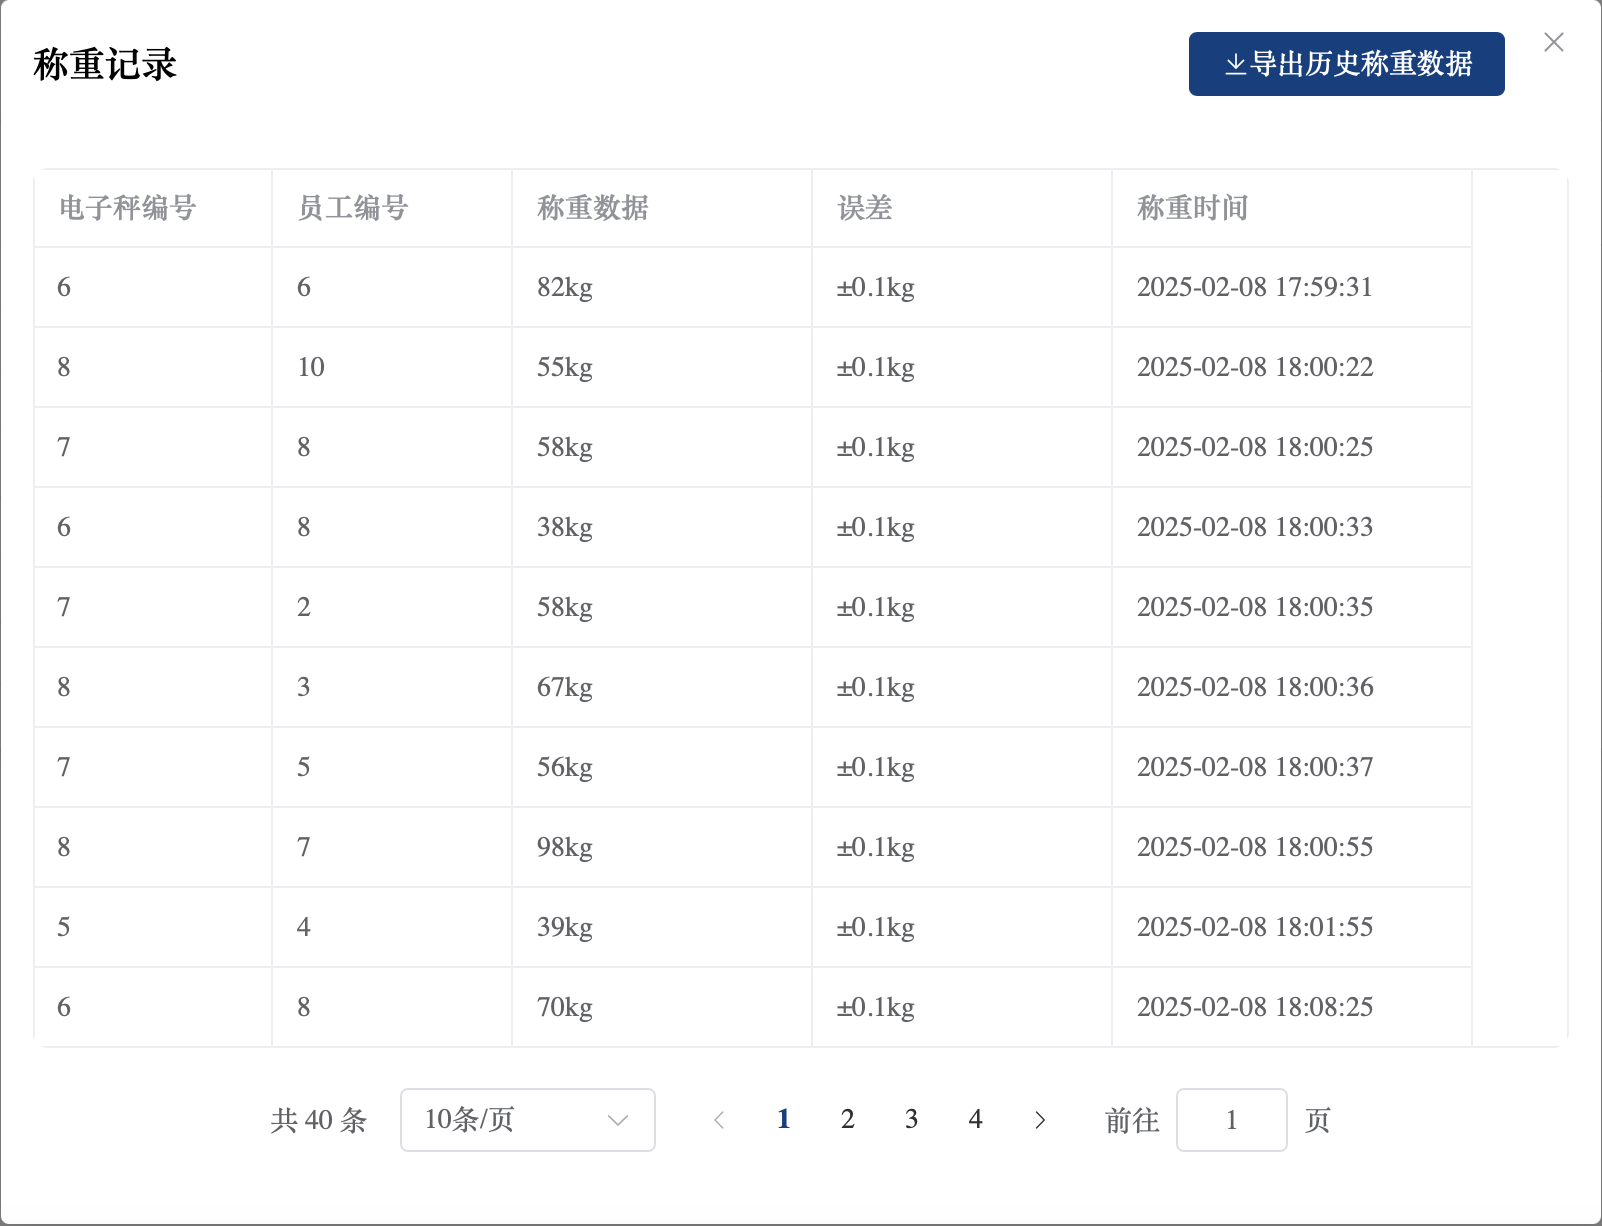
\includegraphics[width=0.8\linewidth]{../result/电子秤称重记录.png}
    \caption{电子秤称重记录}
    \label{fig:电子秤称重记录}
\end{figure}

此外,该界面后续将会支持电子秤终端的模拟操作,实现对称重流程的模拟,支持通过 MQTT、HTTP、CoAP 等协议进行称重数据的提交。

\subsubsection{用户管理模块}

在上方导航处,点击用户模块,进入用户模块界面:

\begin{figure}[H]
    \centering
    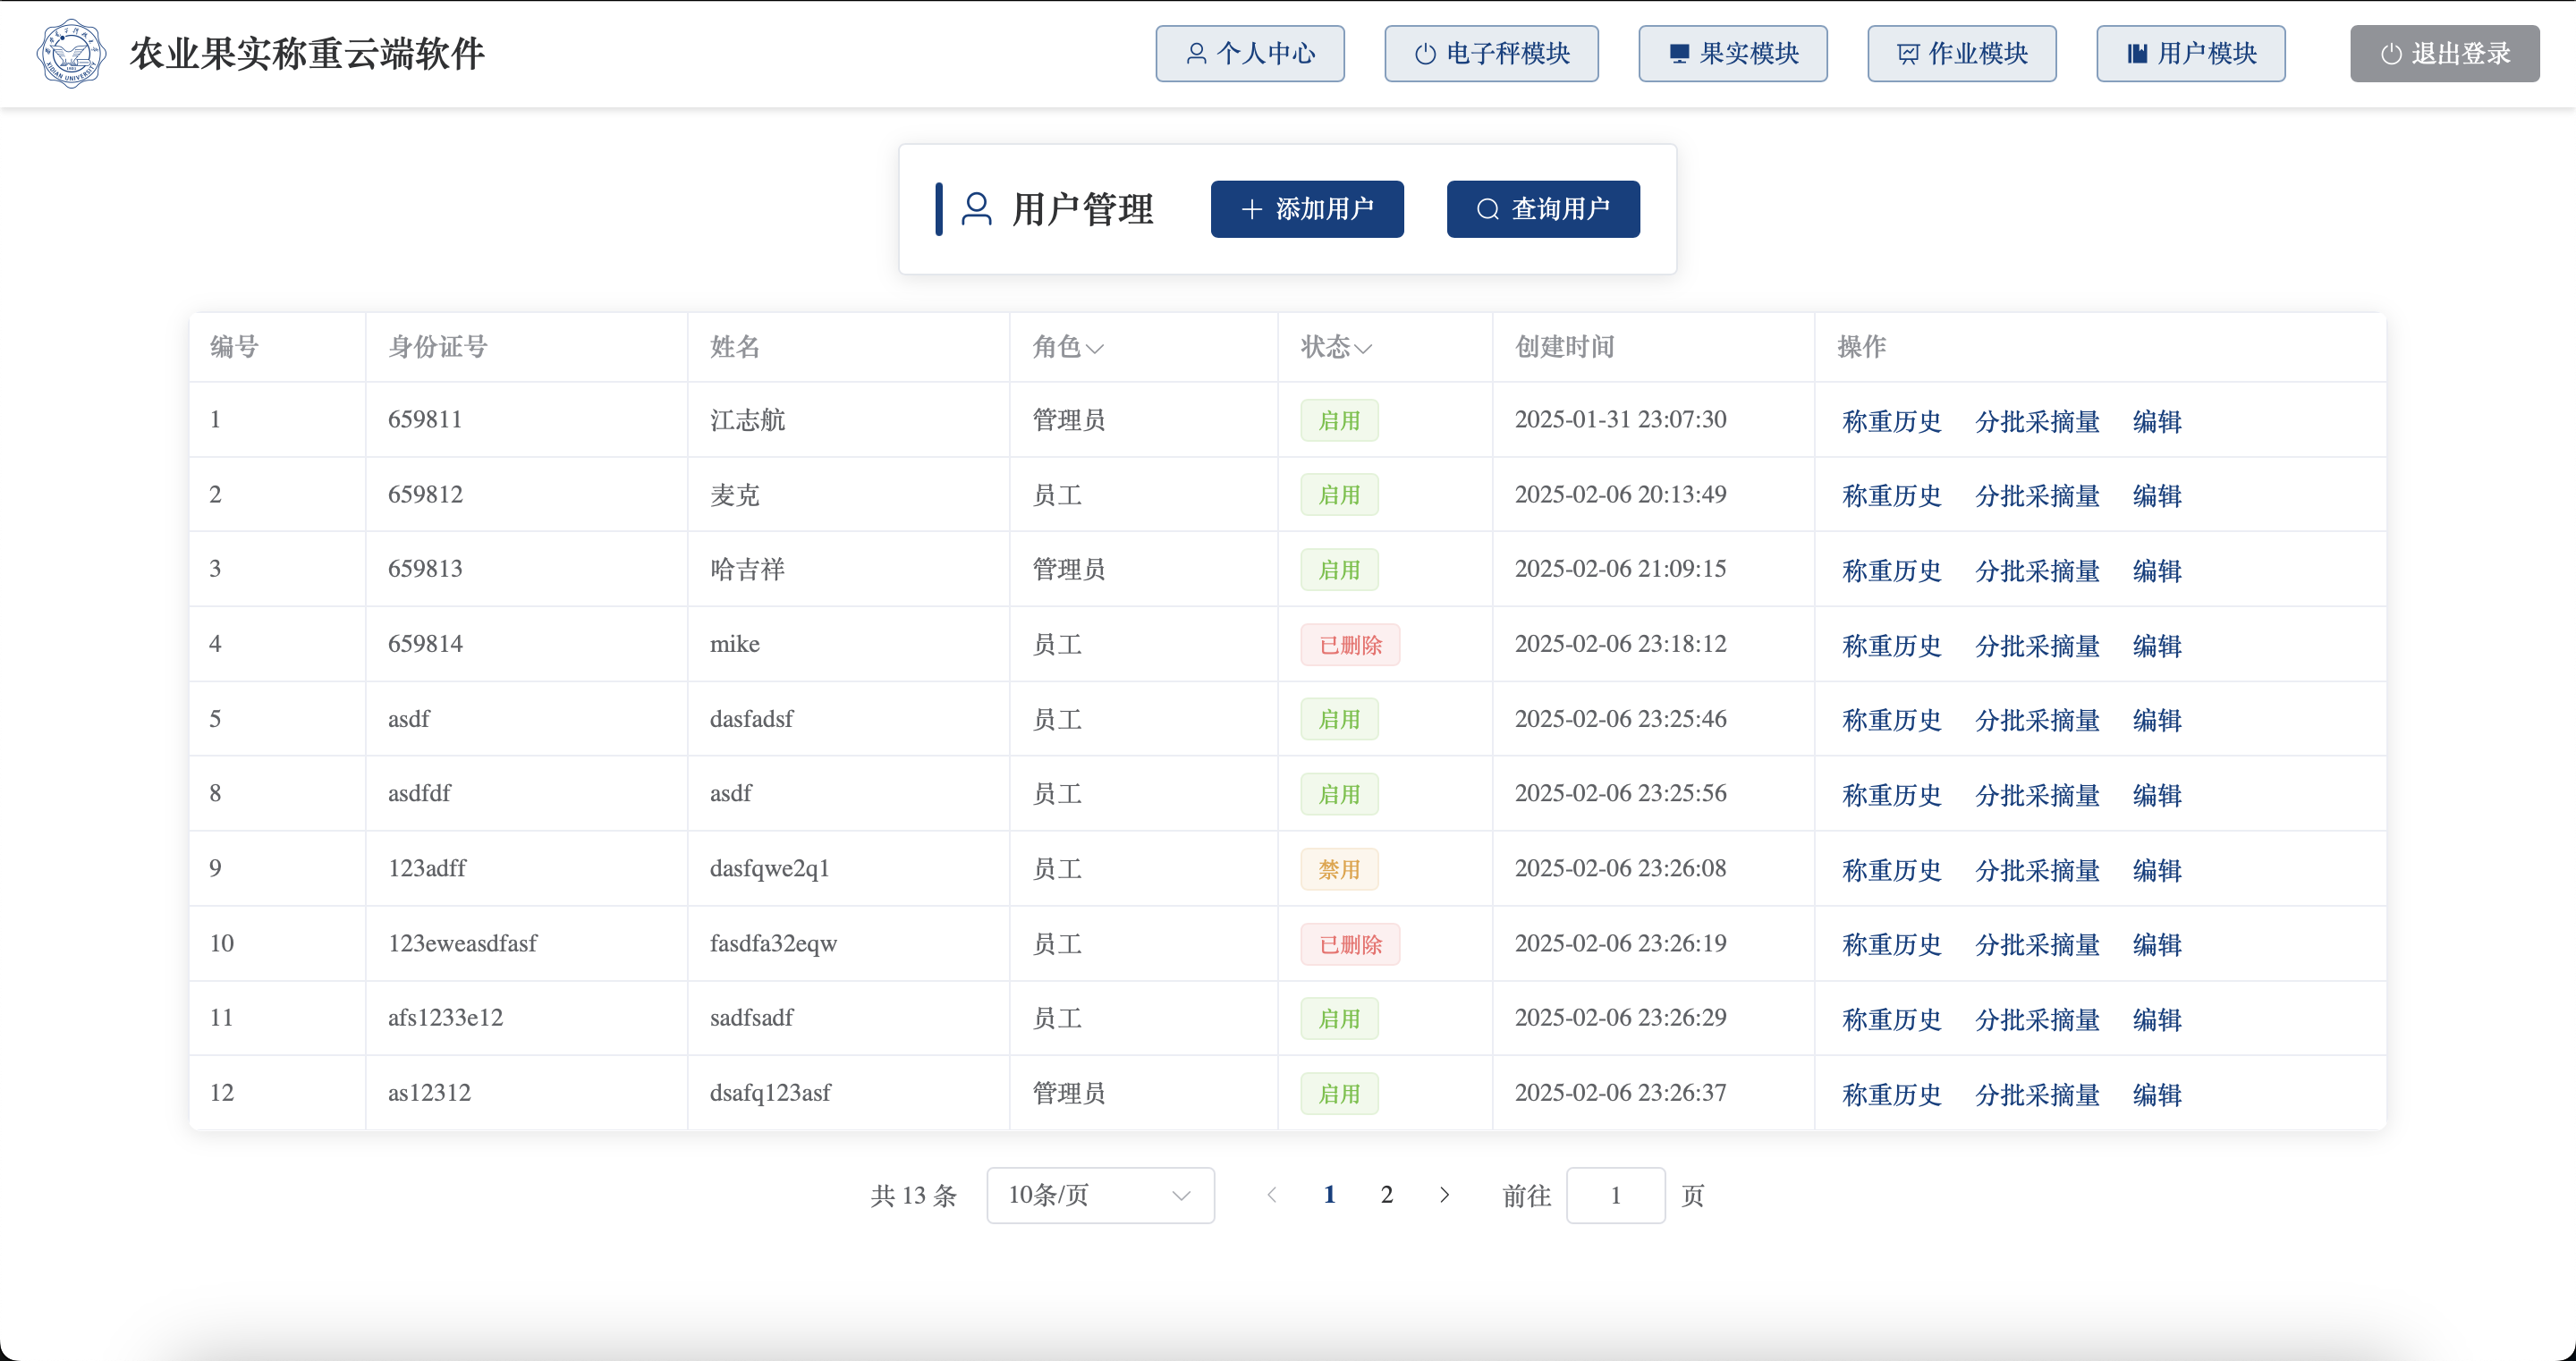
\includegraphics[width=0.8\linewidth]{../result/用户模块.png}
    \caption{用户模块}
    \label{fig:用户模块}
\end{figure}

该界面仅供管理员访问,支持查看、添加、查询和更新员工,也支持查看员工的产出。

\subsubsection{果实管理模块}

在上方导航处,点击果实模块,进入果实模块界面:

\begin{figure}[H]
    \centering
    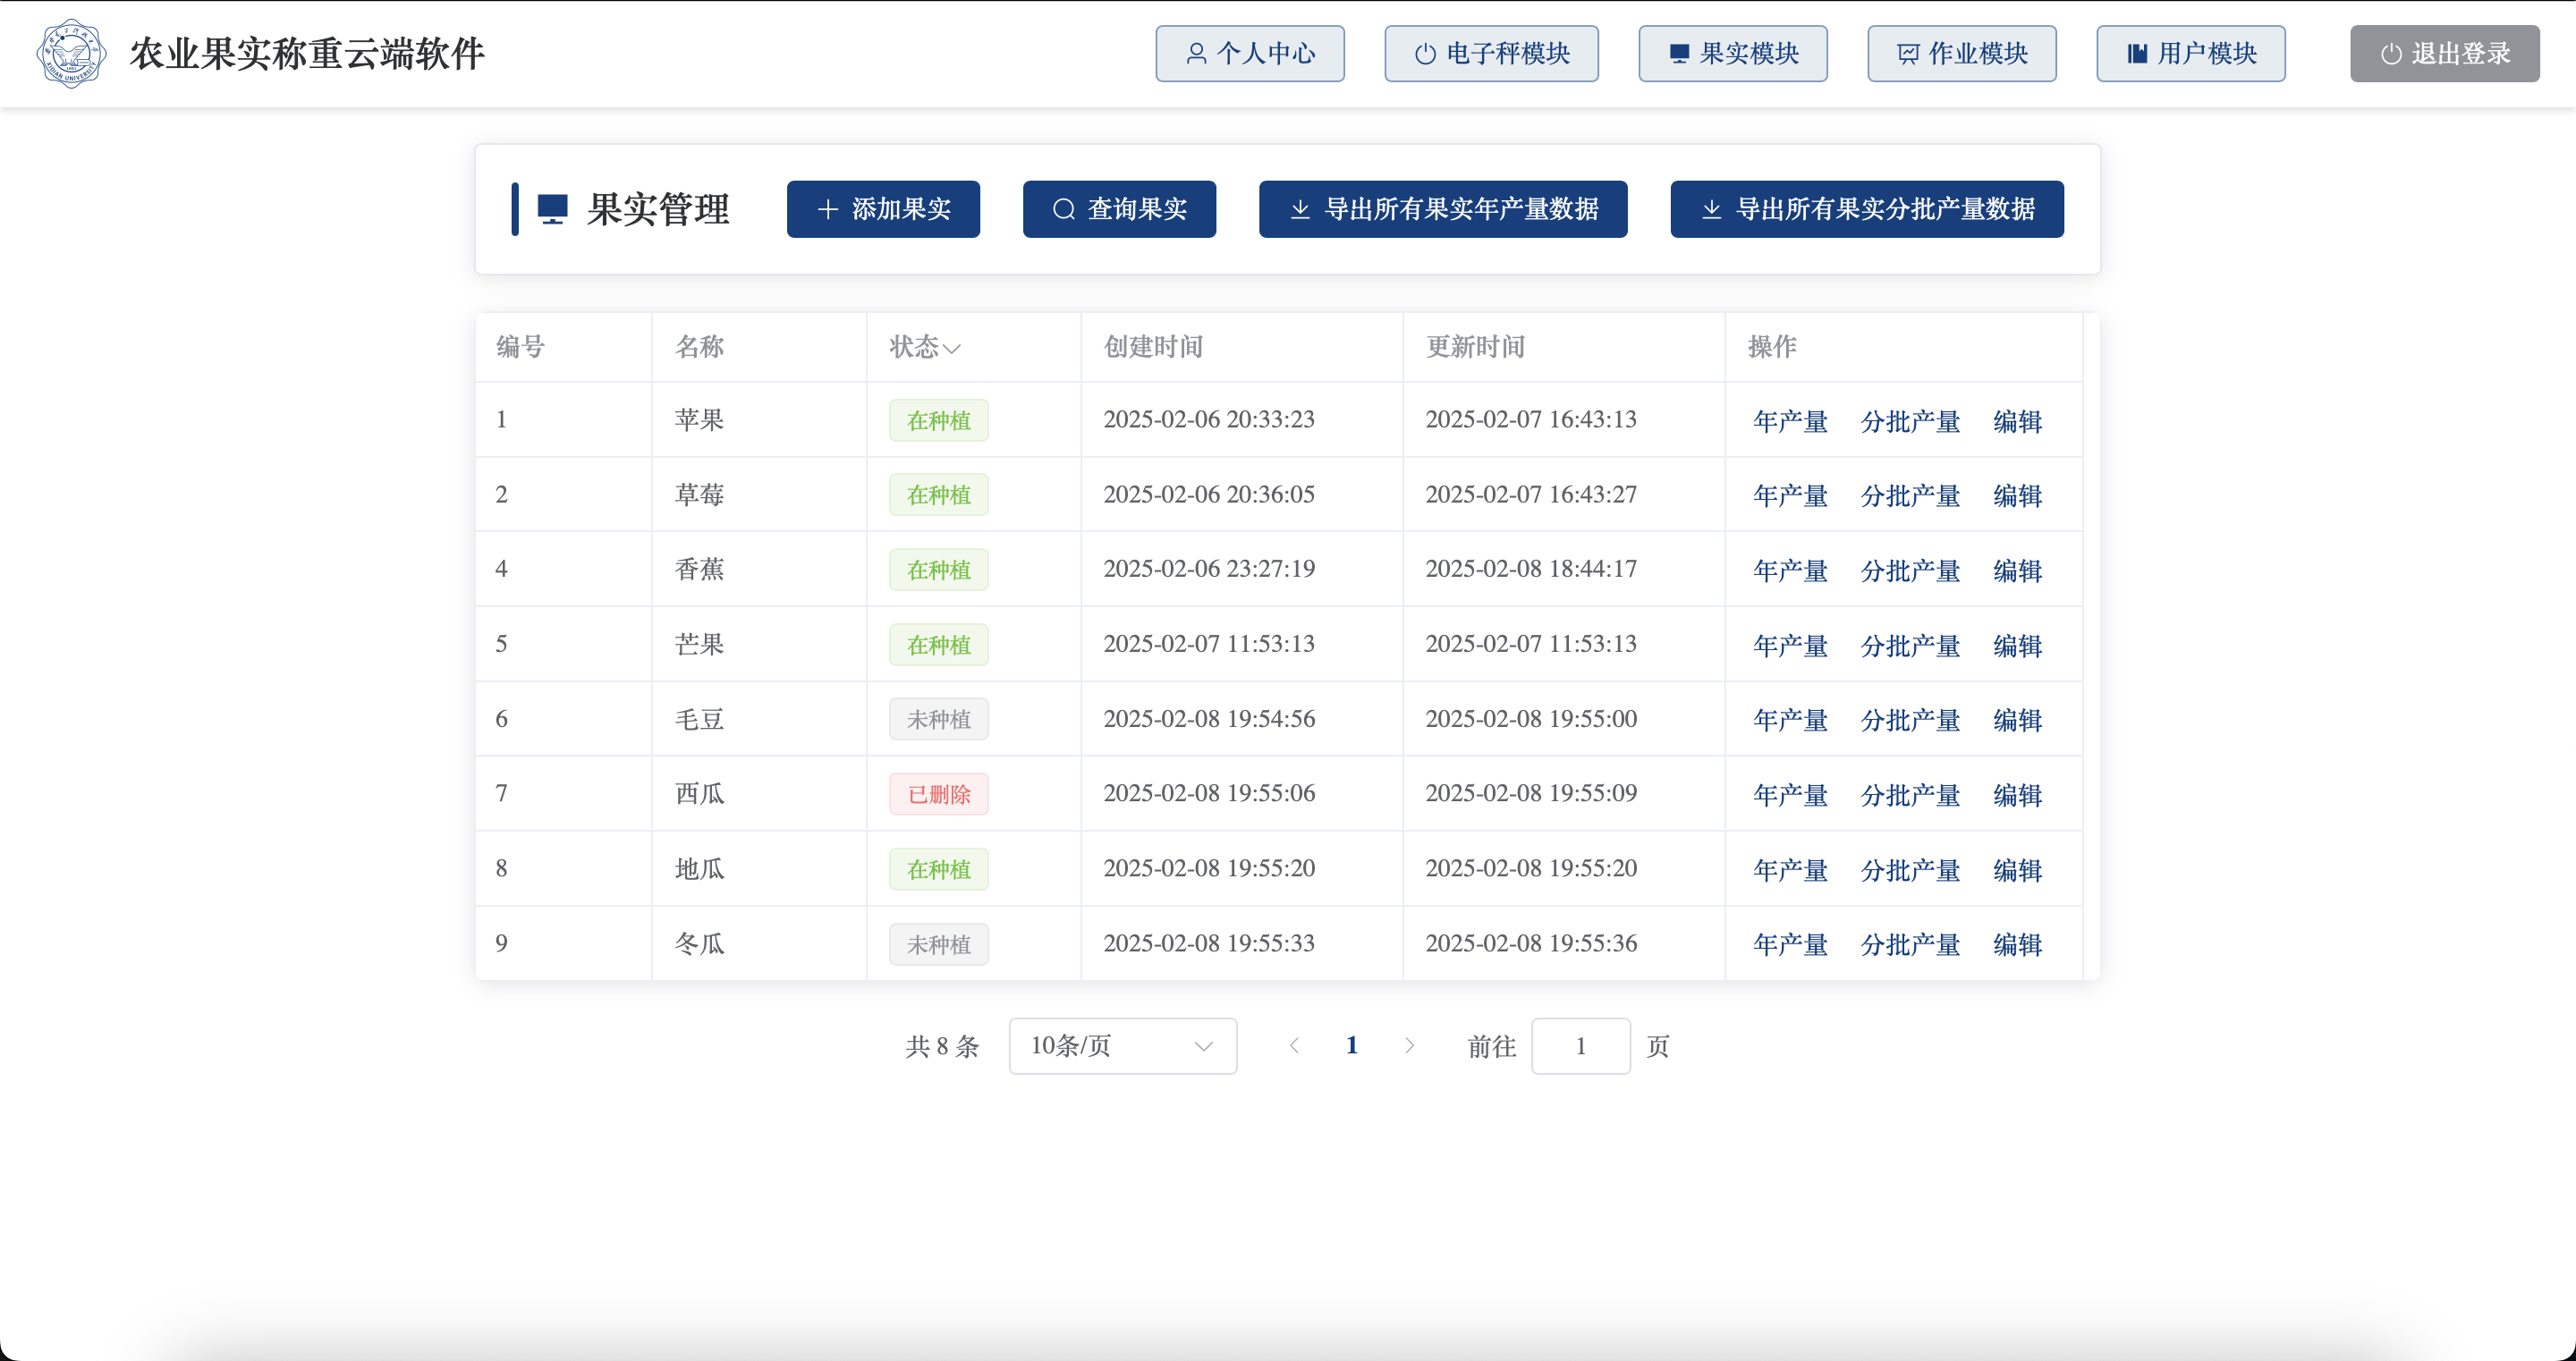
\includegraphics[width=0.8\linewidth]{../result/果实模块.png}
    \caption{果实模块}
    \label{fig:果实模块}
\end{figure}

在该界面中,用户可以对果实执行查看、更新、添加、查询和导出数据等操作。

用户可以点击查看果实分批产量:

\begin{figure}[H]
    \centering
    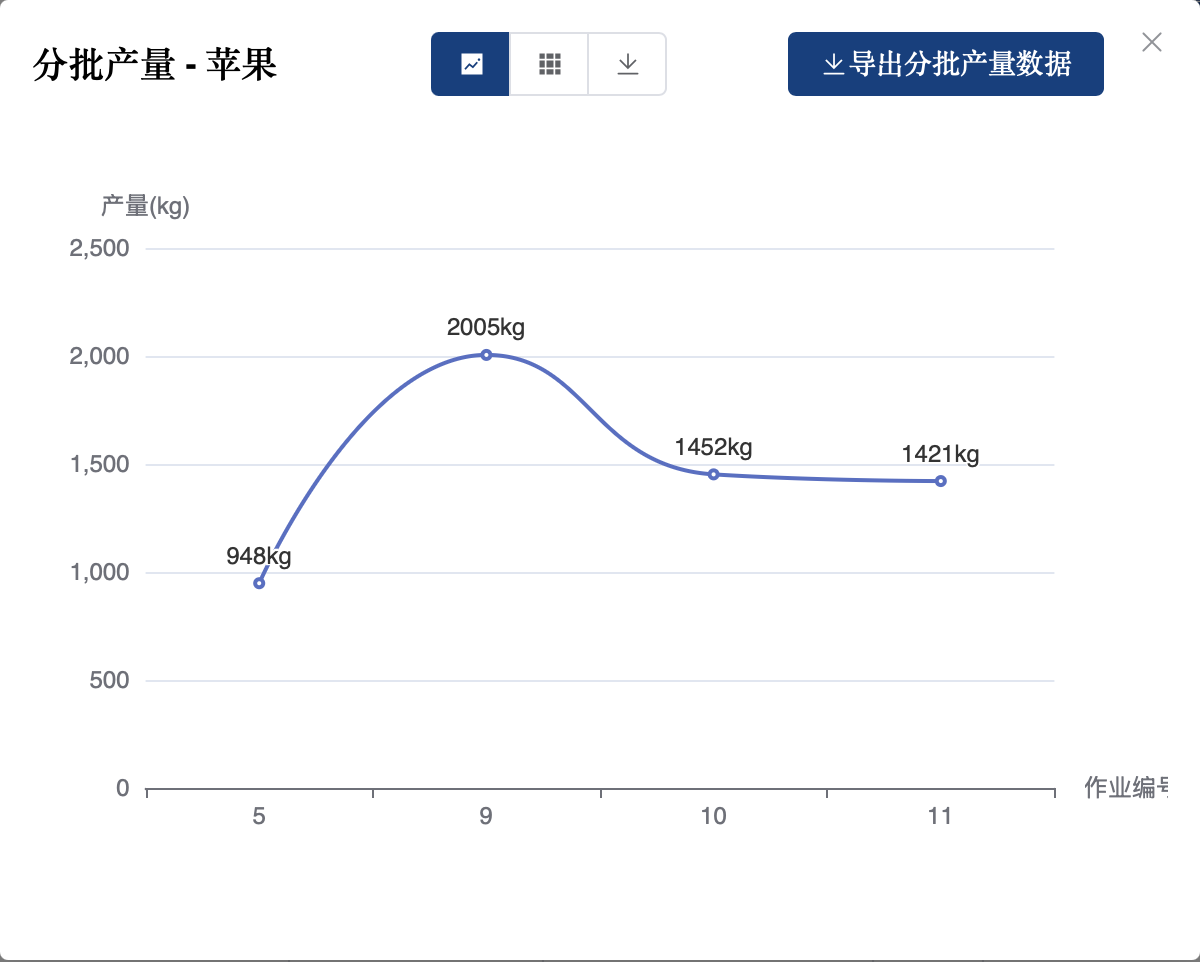
\includegraphics[width=0.8\linewidth]{../result/果实分批产量.png}
    \caption{果实分批产量}
    \label{fig:果实分批产量}
\end{figure}

横坐标为作业编号(批次),纵坐标为产量,单位为 KG。

用户可以点击查看果实年产量:

\begin{figure}[H]
    \centering
    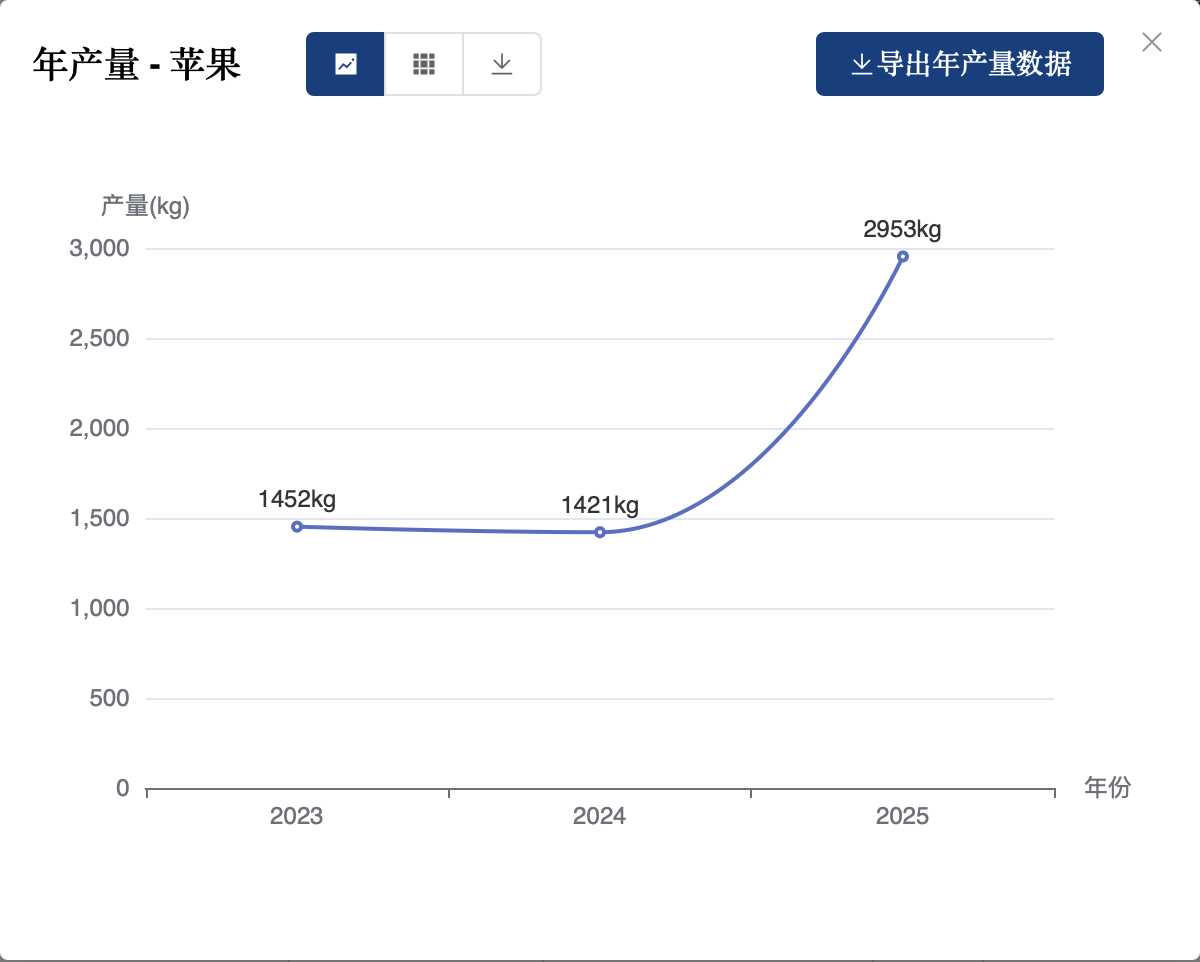
\includegraphics[width=0.8\linewidth]{../result/果实年产量.png}
    \caption{果实年产量}
    \label{fig:果实年产量}
\end{figure}

横坐标为年份,纵坐标为产量,单位为 KG。

\section{后期拟完成的研究工作及进度安排(要有可行性)}

\begin{enumerate}
    \item 第九周:完成电子秤终端模拟器的开发和相关论文编写
    \item 第十周:优化前后台系统,让功能更加完善,比如优化接口性能、优化前台界面展现等
    \item 第十一周:完成系统测试,包括接口测试、压力测试等,然后完成相关论文编写
    \item 第十二周及以后:持续润色、完善论文,正式答辩前完成论文编写
\end{enumerate}

\section{存在的困难与问题}
\begin{enumerate}
    \item 对前台开发不够熟悉,前台代码出现较多冗余,设计不够合理,优化空间很大,后续如果有时间,将会进行重构;
    \item 对压力测试计划的设计存在困难,没有做过相关压力测试的经验,对压力测试根据 Jmeter 不够熟悉,需要借鉴相关项目的测试计划来完成;
    \item 对物联网协议网关的设计不够细致,部分协议转换到 MQTT 可能存在安全性问题,这是由于协议之间的设计差异导致的,后续需要想办法进行优化。
\end{enumerate}

\section{如期完成全部论文工作的可能性}
可以如期完成全部论文工作。

\end{document}